\documentclass[11pt]{article}
\usepackage[T2A]{fontenc}
\usepackage[utf8]{inputenc}
\usepackage[english,russian]{babel}
    \usepackage[breakable]{tcolorbox}
    \usepackage{parskip} % Stop auto-indenting (to mimic markdown behaviour)
    

    % Basic figure setup, for now with no caption control since it's done
    % automatically by Pandoc (which extracts ![](path) syntax from Markdown).
    \usepackage{graphicx}
    % Maintain compatibility with old templates. Remove in nbconvert 6.0
    \let\Oldincludegraphics\includegraphics
    % Ensure that by default, figures have no caption (until we provide a
    % proper Figure object with a Caption API and a way to capture that
    % in the conversion process - todo).
    \usepackage{caption}
    \DeclareCaptionFormat{nocaption}{}
    \captionsetup{format=nocaption,aboveskip=0pt,belowskip=0pt}

    \usepackage{float}
    \floatplacement{figure}{H} % forces figures to be placed at the correct location
    \usepackage{xcolor} % Allow colors to be defined
    \usepackage{enumerate} % Needed for markdown enumerations to work
    \usepackage{geometry} % Used to adjust the document margins
    \usepackage{amsmath} % Equations
    \usepackage{amssymb} % Equations
    \usepackage{textcomp} % defines textquotesingle
    % Hack from http://tex.stackexchange.com/a/47451/13684:
    \AtBeginDocument{%
        \def\PYZsq{\textquotesingle}% Upright quotes in Pygmentized code
    }
    \usepackage{upquote} % Upright quotes for verbatim code
    \usepackage{eurosym} % defines \euro

    \usepackage{iftex}
    \ifPDFTeX
        \usepackage[T1]{fontenc}
        \IfFileExists{alphabeta.sty}{
              \usepackage{alphabeta}
          }{
              \usepackage[mathletters]{ucs}
              \usepackage[utf8x]{inputenc}
          }
    \else
        \usepackage{fontspec}
        \usepackage{unicode-math}
    \fi

    \usepackage{fancyvrb} % verbatim replacement that allows latex
    \usepackage{grffile} % extends the file name processing of package graphics
                         % to support a larger range
    \makeatletter % fix for old versions of grffile with XeLaTeX
    \@ifpackagelater{grffile}{2019/11/01}
    {
      % Do nothing on new versions
    }
    {
      \def\Gread@@xetex#1{%
        \IfFileExists{"\Gin@base".bb}%
        {\Gread@eps{\Gin@base.bb}}%
        {\Gread@@xetex@aux#1}%
      }
    }
    \makeatother
    \usepackage[Export]{adjustbox} % Used to constrain images to a maximum size
    \adjustboxset{max size={0.9\linewidth}{0.9\paperheight}}

    % The hyperref package gives us a pdf with properly built
    % internal navigation ('pdf bookmarks' for the table of contents,
    % internal cross-reference links, web links for URLs, etc.)
    \usepackage{hyperref}
    % The default LaTeX title has an obnoxious amount of whitespace. By default,
    % titling removes some of it. It also provides customization options.
    \usepackage{titling}
    \usepackage{longtable} % longtable support required by pandoc >1.10
    \usepackage{booktabs}  % table support for pandoc > 1.12.2
    \usepackage{array}     % table support for pandoc >= 2.11.3
    \usepackage{calc}      % table minipage width calculation for pandoc >= 2.11.1
    \usepackage[inline]{enumitem} % IRkernel/repr support (it uses the enumerate* environment)
    \usepackage[normalem]{ulem} % ulem is needed to support strikethroughs (\sout)
                                % normalem makes italics be italics, not underlines
    \usepackage{mathrsfs}
    

    
    % Colors for the hyperref package
    \definecolor{urlcolor}{rgb}{0,.145,.698}
    \definecolor{linkcolor}{rgb}{.71,0.21,0.01}
    \definecolor{citecolor}{rgb}{.12,.54,.11}

    % ANSI colors
    \definecolor{ansi-black}{HTML}{3E424D}
    \definecolor{ansi-black-intense}{HTML}{282C36}
    \definecolor{ansi-red}{HTML}{E75C58}
    \definecolor{ansi-red-intense}{HTML}{B22B31}
    \definecolor{ansi-green}{HTML}{00A250}
    \definecolor{ansi-green-intense}{HTML}{007427}
    \definecolor{ansi-yellow}{HTML}{DDB62B}
    \definecolor{ansi-yellow-intense}{HTML}{B27D12}
    \definecolor{ansi-blue}{HTML}{208FFB}
    \definecolor{ansi-blue-intense}{HTML}{0065CA}
    \definecolor{ansi-magenta}{HTML}{D160C4}
    \definecolor{ansi-magenta-intense}{HTML}{A03196}
    \definecolor{ansi-cyan}{HTML}{60C6C8}
    \definecolor{ansi-cyan-intense}{HTML}{258F8F}
    \definecolor{ansi-white}{HTML}{C5C1B4}
    \definecolor{ansi-white-intense}{HTML}{A1A6B2}
    \definecolor{ansi-default-inverse-fg}{HTML}{FFFFFF}
    \definecolor{ansi-default-inverse-bg}{HTML}{000000}

    % common color for the border for error outputs.
    \definecolor{outerrorbackground}{HTML}{FFDFDF}

    % commands and environments needed by pandoc snippets
    % extracted from the output of `pandoc -s`
    \providecommand{\tightlist}{%
      \setlength{\itemsep}{0pt}\setlength{\parskip}{0pt}}
    \DefineVerbatimEnvironment{Highlighting}{Verbatim}{commandchars=\\\{\}}
    % Add ',fontsize=\small' for more characters per line
    \newenvironment{Shaded}{}{}
    \newcommand{\KeywordTok}[1]{\textcolor[rgb]{0.00,0.44,0.13}{\textbf{{#1}}}}
    \newcommand{\DataTypeTok}[1]{\textcolor[rgb]{0.56,0.13,0.00}{{#1}}}
    \newcommand{\DecValTok}[1]{\textcolor[rgb]{0.25,0.63,0.44}{{#1}}}
    \newcommand{\BaseNTok}[1]{\textcolor[rgb]{0.25,0.63,0.44}{{#1}}}
    \newcommand{\FloatTok}[1]{\textcolor[rgb]{0.25,0.63,0.44}{{#1}}}
    \newcommand{\CharTok}[1]{\textcolor[rgb]{0.25,0.44,0.63}{{#1}}}
    \newcommand{\StringTok}[1]{\textcolor[rgb]{0.25,0.44,0.63}{{#1}}}
    \newcommand{\CommentTok}[1]{\textcolor[rgb]{0.38,0.63,0.69}{\textit{{#1}}}}
    \newcommand{\OtherTok}[1]{\textcolor[rgb]{0.00,0.44,0.13}{{#1}}}
    \newcommand{\AlertTok}[1]{\textcolor[rgb]{1.00,0.00,0.00}{\textbf{{#1}}}}
    \newcommand{\FunctionTok}[1]{\textcolor[rgb]{0.02,0.16,0.49}{{#1}}}
    \newcommand{\RegionMarkerTok}[1]{{#1}}
    \newcommand{\ErrorTok}[1]{\textcolor[rgb]{1.00,0.00,0.00}{\textbf{{#1}}}}
    \newcommand{\NormalTok}[1]{{#1}}

    % Additional commands for more recent versions of Pandoc
    \newcommand{\ConstantTok}[1]{\textcolor[rgb]{0.53,0.00,0.00}{{#1}}}
    \newcommand{\SpecialCharTok}[1]{\textcolor[rgb]{0.25,0.44,0.63}{{#1}}}
    \newcommand{\VerbatimStringTok}[1]{\textcolor[rgb]{0.25,0.44,0.63}{{#1}}}
    \newcommand{\SpecialStringTok}[1]{\textcolor[rgb]{0.73,0.40,0.53}{{#1}}}
    \newcommand{\ImportTok}[1]{{#1}}
    \newcommand{\DocumentationTok}[1]{\textcolor[rgb]{0.73,0.13,0.13}{\textit{{#1}}}}
    \newcommand{\AnnotationTok}[1]{\textcolor[rgb]{0.38,0.63,0.69}{\textbf{\textit{{#1}}}}}
    \newcommand{\CommentVarTok}[1]{\textcolor[rgb]{0.38,0.63,0.69}{\textbf{\textit{{#1}}}}}
    \newcommand{\VariableTok}[1]{\textcolor[rgb]{0.10,0.09,0.49}{{#1}}}
    \newcommand{\ControlFlowTok}[1]{\textcolor[rgb]{0.00,0.44,0.13}{\textbf{{#1}}}}
    \newcommand{\OperatorTok}[1]{\textcolor[rgb]{0.40,0.40,0.40}{{#1}}}
    \newcommand{\BuiltInTok}[1]{{#1}}
    \newcommand{\ExtensionTok}[1]{{#1}}
    \newcommand{\PreprocessorTok}[1]{\textcolor[rgb]{0.74,0.48,0.00}{{#1}}}
    \newcommand{\AttributeTok}[1]{\textcolor[rgb]{0.49,0.56,0.16}{{#1}}}
    \newcommand{\InformationTok}[1]{\textcolor[rgb]{0.38,0.63,0.69}{\textbf{\textit{{#1}}}}}
    \newcommand{\WarningTok}[1]{\textcolor[rgb]{0.38,0.63,0.69}{\textbf{\textit{{#1}}}}}


    % Define a nice break command that doesn't care if a line doesn't already
    % exist.
    \def\br{\hspace*{\fill} \\* }
    % Math Jax compatibility definitions
    \def\gt{>}
    \def\lt{<}
    \let\Oldtex\TeX
    \let\Oldlatex\LaTeX
    \renewcommand{\TeX}{\textrm{\Oldtex}}
    \renewcommand{\LaTeX}{\textrm{\Oldlatex}}
    % Document parameters
    % Document title
    \title{7-8}
    
    
    
    
    
% Pygments definitions
\makeatletter
\def\PY@reset{\let\PY@it=\relax \let\PY@bf=\relax%
    \let\PY@ul=\relax \let\PY@tc=\relax%
    \let\PY@bc=\relax \let\PY@ff=\relax}
\def\PY@tok#1{\csname PY@tok@#1\endcsname}
\def\PY@toks#1+{\ifx\relax#1\empty\else%
    \PY@tok{#1}\expandafter\PY@toks\fi}
\def\PY@do#1{\PY@bc{\PY@tc{\PY@ul{%
    \PY@it{\PY@bf{\PY@ff{#1}}}}}}}
\def\PY#1#2{\PY@reset\PY@toks#1+\relax+\PY@do{#2}}

\@namedef{PY@tok@w}{\def\PY@tc##1{\textcolor[rgb]{0.73,0.73,0.73}{##1}}}
\@namedef{PY@tok@c}{\let\PY@it=\textit\def\PY@tc##1{\textcolor[rgb]{0.24,0.48,0.48}{##1}}}
\@namedef{PY@tok@cp}{\def\PY@tc##1{\textcolor[rgb]{0.61,0.40,0.00}{##1}}}
\@namedef{PY@tok@k}{\let\PY@bf=\textbf\def\PY@tc##1{\textcolor[rgb]{0.00,0.50,0.00}{##1}}}
\@namedef{PY@tok@kp}{\def\PY@tc##1{\textcolor[rgb]{0.00,0.50,0.00}{##1}}}
\@namedef{PY@tok@kt}{\def\PY@tc##1{\textcolor[rgb]{0.69,0.00,0.25}{##1}}}
\@namedef{PY@tok@o}{\def\PY@tc##1{\textcolor[rgb]{0.40,0.40,0.40}{##1}}}
\@namedef{PY@tok@ow}{\let\PY@bf=\textbf\def\PY@tc##1{\textcolor[rgb]{0.67,0.13,1.00}{##1}}}
\@namedef{PY@tok@nb}{\def\PY@tc##1{\textcolor[rgb]{0.00,0.50,0.00}{##1}}}
\@namedef{PY@tok@nf}{\def\PY@tc##1{\textcolor[rgb]{0.00,0.00,1.00}{##1}}}
\@namedef{PY@tok@nc}{\let\PY@bf=\textbf\def\PY@tc##1{\textcolor[rgb]{0.00,0.00,1.00}{##1}}}
\@namedef{PY@tok@nn}{\let\PY@bf=\textbf\def\PY@tc##1{\textcolor[rgb]{0.00,0.00,1.00}{##1}}}
\@namedef{PY@tok@ne}{\let\PY@bf=\textbf\def\PY@tc##1{\textcolor[rgb]{0.80,0.25,0.22}{##1}}}
\@namedef{PY@tok@nv}{\def\PY@tc##1{\textcolor[rgb]{0.10,0.09,0.49}{##1}}}
\@namedef{PY@tok@no}{\def\PY@tc##1{\textcolor[rgb]{0.53,0.00,0.00}{##1}}}
\@namedef{PY@tok@nl}{\def\PY@tc##1{\textcolor[rgb]{0.46,0.46,0.00}{##1}}}
\@namedef{PY@tok@ni}{\let\PY@bf=\textbf\def\PY@tc##1{\textcolor[rgb]{0.44,0.44,0.44}{##1}}}
\@namedef{PY@tok@na}{\def\PY@tc##1{\textcolor[rgb]{0.41,0.47,0.13}{##1}}}
\@namedef{PY@tok@nt}{\let\PY@bf=\textbf\def\PY@tc##1{\textcolor[rgb]{0.00,0.50,0.00}{##1}}}
\@namedef{PY@tok@nd}{\def\PY@tc##1{\textcolor[rgb]{0.67,0.13,1.00}{##1}}}
\@namedef{PY@tok@s}{\def\PY@tc##1{\textcolor[rgb]{0.73,0.13,0.13}{##1}}}
\@namedef{PY@tok@sd}{\let\PY@it=\textit\def\PY@tc##1{\textcolor[rgb]{0.73,0.13,0.13}{##1}}}
\@namedef{PY@tok@si}{\let\PY@bf=\textbf\def\PY@tc##1{\textcolor[rgb]{0.64,0.35,0.47}{##1}}}
\@namedef{PY@tok@se}{\let\PY@bf=\textbf\def\PY@tc##1{\textcolor[rgb]{0.67,0.36,0.12}{##1}}}
\@namedef{PY@tok@sr}{\def\PY@tc##1{\textcolor[rgb]{0.64,0.35,0.47}{##1}}}
\@namedef{PY@tok@ss}{\def\PY@tc##1{\textcolor[rgb]{0.10,0.09,0.49}{##1}}}
\@namedef{PY@tok@sx}{\def\PY@tc##1{\textcolor[rgb]{0.00,0.50,0.00}{##1}}}
\@namedef{PY@tok@m}{\def\PY@tc##1{\textcolor[rgb]{0.40,0.40,0.40}{##1}}}
\@namedef{PY@tok@gh}{\let\PY@bf=\textbf\def\PY@tc##1{\textcolor[rgb]{0.00,0.00,0.50}{##1}}}
\@namedef{PY@tok@gu}{\let\PY@bf=\textbf\def\PY@tc##1{\textcolor[rgb]{0.50,0.00,0.50}{##1}}}
\@namedef{PY@tok@gd}{\def\PY@tc##1{\textcolor[rgb]{0.63,0.00,0.00}{##1}}}
\@namedef{PY@tok@gi}{\def\PY@tc##1{\textcolor[rgb]{0.00,0.52,0.00}{##1}}}
\@namedef{PY@tok@gr}{\def\PY@tc##1{\textcolor[rgb]{0.89,0.00,0.00}{##1}}}
\@namedef{PY@tok@ge}{\let\PY@it=\textit}
\@namedef{PY@tok@gs}{\let\PY@bf=\textbf}
\@namedef{PY@tok@gp}{\let\PY@bf=\textbf\def\PY@tc##1{\textcolor[rgb]{0.00,0.00,0.50}{##1}}}
\@namedef{PY@tok@go}{\def\PY@tc##1{\textcolor[rgb]{0.44,0.44,0.44}{##1}}}
\@namedef{PY@tok@gt}{\def\PY@tc##1{\textcolor[rgb]{0.00,0.27,0.87}{##1}}}
\@namedef{PY@tok@err}{\def\PY@bc##1{{\setlength{\fboxsep}{\string -\fboxrule}\fcolorbox[rgb]{1.00,0.00,0.00}{1,1,1}{\strut ##1}}}}
\@namedef{PY@tok@kc}{\let\PY@bf=\textbf\def\PY@tc##1{\textcolor[rgb]{0.00,0.50,0.00}{##1}}}
\@namedef{PY@tok@kd}{\let\PY@bf=\textbf\def\PY@tc##1{\textcolor[rgb]{0.00,0.50,0.00}{##1}}}
\@namedef{PY@tok@kn}{\let\PY@bf=\textbf\def\PY@tc##1{\textcolor[rgb]{0.00,0.50,0.00}{##1}}}
\@namedef{PY@tok@kr}{\let\PY@bf=\textbf\def\PY@tc##1{\textcolor[rgb]{0.00,0.50,0.00}{##1}}}
\@namedef{PY@tok@bp}{\def\PY@tc##1{\textcolor[rgb]{0.00,0.50,0.00}{##1}}}
\@namedef{PY@tok@fm}{\def\PY@tc##1{\textcolor[rgb]{0.00,0.00,1.00}{##1}}}
\@namedef{PY@tok@vc}{\def\PY@tc##1{\textcolor[rgb]{0.10,0.09,0.49}{##1}}}
\@namedef{PY@tok@vg}{\def\PY@tc##1{\textcolor[rgb]{0.10,0.09,0.49}{##1}}}
\@namedef{PY@tok@vi}{\def\PY@tc##1{\textcolor[rgb]{0.10,0.09,0.49}{##1}}}
\@namedef{PY@tok@vm}{\def\PY@tc##1{\textcolor[rgb]{0.10,0.09,0.49}{##1}}}
\@namedef{PY@tok@sa}{\def\PY@tc##1{\textcolor[rgb]{0.73,0.13,0.13}{##1}}}
\@namedef{PY@tok@sb}{\def\PY@tc##1{\textcolor[rgb]{0.73,0.13,0.13}{##1}}}
\@namedef{PY@tok@sc}{\def\PY@tc##1{\textcolor[rgb]{0.73,0.13,0.13}{##1}}}
\@namedef{PY@tok@dl}{\def\PY@tc##1{\textcolor[rgb]{0.73,0.13,0.13}{##1}}}
\@namedef{PY@tok@s2}{\def\PY@tc##1{\textcolor[rgb]{0.73,0.13,0.13}{##1}}}
\@namedef{PY@tok@sh}{\def\PY@tc##1{\textcolor[rgb]{0.73,0.13,0.13}{##1}}}
\@namedef{PY@tok@s1}{\def\PY@tc##1{\textcolor[rgb]{0.73,0.13,0.13}{##1}}}
\@namedef{PY@tok@mb}{\def\PY@tc##1{\textcolor[rgb]{0.40,0.40,0.40}{##1}}}
\@namedef{PY@tok@mf}{\def\PY@tc##1{\textcolor[rgb]{0.40,0.40,0.40}{##1}}}
\@namedef{PY@tok@mh}{\def\PY@tc##1{\textcolor[rgb]{0.40,0.40,0.40}{##1}}}
\@namedef{PY@tok@mi}{\def\PY@tc##1{\textcolor[rgb]{0.40,0.40,0.40}{##1}}}
\@namedef{PY@tok@il}{\def\PY@tc##1{\textcolor[rgb]{0.40,0.40,0.40}{##1}}}
\@namedef{PY@tok@mo}{\def\PY@tc##1{\textcolor[rgb]{0.40,0.40,0.40}{##1}}}
\@namedef{PY@tok@ch}{\let\PY@it=\textit\def\PY@tc##1{\textcolor[rgb]{0.24,0.48,0.48}{##1}}}
\@namedef{PY@tok@cm}{\let\PY@it=\textit\def\PY@tc##1{\textcolor[rgb]{0.24,0.48,0.48}{##1}}}
\@namedef{PY@tok@cpf}{\let\PY@it=\textit\def\PY@tc##1{\textcolor[rgb]{0.24,0.48,0.48}{##1}}}
\@namedef{PY@tok@c1}{\let\PY@it=\textit\def\PY@tc##1{\textcolor[rgb]{0.24,0.48,0.48}{##1}}}
\@namedef{PY@tok@cs}{\let\PY@it=\textit\def\PY@tc##1{\textcolor[rgb]{0.24,0.48,0.48}{##1}}}

\def\PYZbs{\char`\\}
\def\PYZus{\char`\_}
\def\PYZob{\char`\{}
\def\PYZcb{\char`\}}
\def\PYZca{\char`\^}
\def\PYZam{\char`\&}
\def\PYZlt{\char`\<}
\def\PYZgt{\char`\>}
\def\PYZsh{\char`\#}
\def\PYZpc{\char`\%}
\def\PYZdl{\char`\$}
\def\PYZhy{\char`\-}
\def\PYZsq{\char`\'}
\def\PYZdq{\char`\"}
\def\PYZti{\char`\~}
% for compatibility with earlier versions
\def\PYZat{@}
\def\PYZlb{[}
\def\PYZrb{]}
\makeatother


    % For linebreaks inside Verbatim environment from package fancyvrb.
    \makeatletter
        \newbox\Wrappedcontinuationbox
        \newbox\Wrappedvisiblespacebox
        \newcommand*\Wrappedvisiblespace {\textcolor{red}{\textvisiblespace}}
        \newcommand*\Wrappedcontinuationsymbol {\textcolor{red}{\llap{\tiny$\m@th\hookrightarrow$}}}
        \newcommand*\Wrappedcontinuationindent {3ex }
        \newcommand*\Wrappedafterbreak {\kern\Wrappedcontinuationindent\copy\Wrappedcontinuationbox}
        % Take advantage of the already applied Pygments mark-up to insert
        % potential linebreaks for TeX processing.
        %        {, <, #, %, $, ' and ": go to next line.
        %        _, }, ^, &, >, - and ~: stay at end of broken line.
        % Use of \textquotesingle for straight quote.
        \newcommand*\Wrappedbreaksatspecials {%
            \def\PYGZus{\discretionary{\char`\_}{\Wrappedafterbreak}{\char`\_}}%
            \def\PYGZob{\discretionary{}{\Wrappedafterbreak\char`\{}{\char`\{}}%
            \def\PYGZcb{\discretionary{\char`\}}{\Wrappedafterbreak}{\char`\}}}%
            \def\PYGZca{\discretionary{\char`\^}{\Wrappedafterbreak}{\char`\^}}%
            \def\PYGZam{\discretionary{\char`\&}{\Wrappedafterbreak}{\char`\&}}%
            \def\PYGZlt{\discretionary{}{\Wrappedafterbreak\char`\<}{\char`\<}}%
            \def\PYGZgt{\discretionary{\char`\>}{\Wrappedafterbreak}{\char`\>}}%
            \def\PYGZsh{\discretionary{}{\Wrappedafterbreak\char`\#}{\char`\#}}%
            \def\PYGZpc{\discretionary{}{\Wrappedafterbreak\char`\%}{\char`\%}}%
            \def\PYGZdl{\discretionary{}{\Wrappedafterbreak\char`\$}{\char`\$}}%
            \def\PYGZhy{\discretionary{\char`\-}{\Wrappedafterbreak}{\char`\-}}%
            \def\PYGZsq{\discretionary{}{\Wrappedafterbreak\textquotesingle}{\textquotesingle}}%
            \def\PYGZdq{\discretionary{}{\Wrappedafterbreak\char`\"}{\char`\"}}%
            \def\PYGZti{\discretionary{\char`\~}{\Wrappedafterbreak}{\char`\~}}%
        }
        % Some characters . , ; ? ! / are not pygmentized.
        % This macro makes them "active" and they will insert potential linebreaks
        \newcommand*\Wrappedbreaksatpunct {%
            \lccode`\~`\.\lowercase{\def~}{\discretionary{\hbox{\char`\.}}{\Wrappedafterbreak}{\hbox{\char`\.}}}%
            \lccode`\~`\,\lowercase{\def~}{\discretionary{\hbox{\char`\,}}{\Wrappedafterbreak}{\hbox{\char`\,}}}%
            \lccode`\~`\;\lowercase{\def~}{\discretionary{\hbox{\char`\;}}{\Wrappedafterbreak}{\hbox{\char`\;}}}%
            \lccode`\~`\:\lowercase{\def~}{\discretionary{\hbox{\char`\:}}{\Wrappedafterbreak}{\hbox{\char`\:}}}%
            \lccode`\~`\?\lowercase{\def~}{\discretionary{\hbox{\char`\?}}{\Wrappedafterbreak}{\hbox{\char`\?}}}%
            \lccode`\~`\!\lowercase{\def~}{\discretionary{\hbox{\char`\!}}{\Wrappedafterbreak}{\hbox{\char`\!}}}%
            \lccode`\~`\/\lowercase{\def~}{\discretionary{\hbox{\char`\/}}{\Wrappedafterbreak}{\hbox{\char`\/}}}%
            \catcode`\.\active
            \catcode`\,\active
            \catcode`\;\active
            \catcode`\:\active
            \catcode`\?\active
            \catcode`\!\active
            \catcode`\/\active
            \lccode`\~`\~
        }
    \makeatother

    \let\OriginalVerbatim=\Verbatim
    \makeatletter
    \renewcommand{\Verbatim}[1][1]{%
        %\parskip\z@skip
        \sbox\Wrappedcontinuationbox {\Wrappedcontinuationsymbol}%
        \sbox\Wrappedvisiblespacebox {\FV@SetupFont\Wrappedvisiblespace}%
        \def\FancyVerbFormatLine ##1{\hsize\linewidth
            \vtop{\raggedright\hyphenpenalty\z@\exhyphenpenalty\z@
                \doublehyphendemerits\z@\finalhyphendemerits\z@
                \strut ##1\strut}%
        }%
        % If the linebreak is at a space, the latter will be displayed as visible
        % space at end of first line, and a continuation symbol starts next line.
        % Stretch/shrink are however usually zero for typewriter font.
        \def\FV@Space {%
            \nobreak\hskip\z@ plus\fontdimen3\font minus\fontdimen4\font
            \discretionary{\copy\Wrappedvisiblespacebox}{\Wrappedafterbreak}
            {\kern\fontdimen2\font}%
        }%

        % Allow breaks at special characters using \PYG... macros.
        \Wrappedbreaksatspecials
        % Breaks at punctuation characters . , ; ? ! and / need catcode=\active
        \OriginalVerbatim[#1,codes*=\Wrappedbreaksatpunct]%
    }
    \makeatother

    % Exact colors from NB
    \definecolor{incolor}{HTML}{303F9F}
    \definecolor{outcolor}{HTML}{D84315}
    \definecolor{cellborder}{HTML}{CFCFCF}
    \definecolor{cellbackground}{HTML}{F7F7F7}

    % prompt
    \makeatletter
    \newcommand{\boxspacing}{\kern\kvtcb@left@rule\kern\kvtcb@boxsep}
    \makeatother
    \newcommand{\prompt}[4]{
        {\ttfamily\llap{{\color{#2}[#3]:\hspace{3pt}#4}}\vspace{-\baselineskip}}
    }
    

    
    % Prevent overflowing lines due to hard-to-break entities
    \sloppy
    % Setup hyperref package
    \hypersetup{
      breaklinks=true,  % so long urls are correctly broken across lines
      colorlinks=true,
      urlcolor=urlcolor,
      linkcolor=linkcolor,
      citecolor=citecolor,
      }
    % Slightly bigger margins than the latex defaults
    
    \geometry{verbose,tmargin=1in,bmargin=1in,lmargin=1in,rmargin=1in}
    
    

\begin{document}
    
    \begin{titlepage}
    	\begin{center}
    		\textsc{МИНИСТЕРСТВО ОБРАЗОВАНИЯ РЕСПУБЛИКИ БЕЛАРУСЬ БЕЛОРУССКИЙ ГОСУДАРСТВЕННЫЙ УНИВЕРСИТЕТ
    			\\[5mm]
    			ФАКУЛЬТЕТ ПРИКЛАДНОЙ МАТЕМАТИКИ И ИНФОРМАТИКИ\\[2mm]
    			Кафедра информационных систем управления
    		}
    		
    		\vfill
    		
    		\textbf{Отчет по лабораторной работе №7-8\\
    			Вариант 2
    			\\[26mm]
    		}
    	\end{center}
    	
    	\hfill
    	\begin{minipage}{.5\textwidth}
    		\begin{flushright}
    			Бовта Тимофея Анатольевича\\
    			студента 3 курса\\
    			специальности «прикладная математика»\\[5mm]
    			
    			Преподаватель:\\[2mm] 
    			Д. Ю. Кваша\\
    		\end{flushright}
    	\end{minipage}%
    	\vfill
    	\begin{center}
    		Минск, 2024\ г.
    	\end{center}
    \end{titlepage}
    
    

    
    \section{Задача 1}\label{ux437ux430ux434ux430ux447ux430-1}

    Найдите решение игры заданной матрицей
\[A = \begin{bmatrix} 3 & 4 \\ 5 & 1 \end{bmatrix}\]

    Нижняя цена игры:
\[\alpha(A)=\max\limits_{1\leq j\leq 2}\min\limits_{1\leq i\leq 2}a_{ij}=3.\]
Верхняя цена игры:
\[\beta(A)=\min\limits_{1\leq i\leq 2}\max\limits_{1\leq j\leq 2}a_{ij}=4.\]
Таким образом, \(\alpha(A)\neq \beta(A)\).

Реализуем программно данную проверку:

    \begin{tcolorbox}[breakable, size=fbox, boxrule=1pt, pad at break*=1mm,colback=cellbackground, colframe=cellborder]
\prompt{In}{incolor}{39}{\boxspacing}
\begin{Verbatim}[commandchars=\\\{\}]
\PY{k+kn}{import} \PY{n+nn}{numpy} \PY{k}{as} \PY{n+nn}{np}
\PY{n}{A} \PY{o}{=} \PY{n}{np}\PY{o}{.}\PY{n}{array}\PY{p}{(}\PY{p}{[}\PY{p}{[}\PY{l+m+mi}{3}\PY{p}{,} \PY{l+m+mi}{4}\PY{p}{]}\PY{p}{,} \PY{p}{[}\PY{l+m+mi}{5}\PY{p}{,} \PY{l+m+mi}{1}\PY{p}{]}\PY{p}{]}\PY{p}{)}

\PY{k}{def} \PY{n+nf}{lower\PYZus{}bound\PYZus{}price}\PY{p}{(}\PY{n}{A}\PY{p}{)}\PY{p}{:}
        \PY{k}{return} \PY{n}{A}\PY{o}{.}\PY{n}{min}\PY{p}{(}\PY{n}{axis}\PY{o}{=}\PY{l+m+mi}{1}\PY{p}{)}\PY{o}{.}\PY{n}{max}\PY{p}{(}\PY{p}{)}
    
\PY{k}{def} \PY{n+nf}{upper\PYZus{}bound\PYZus{}price}\PY{p}{(}\PY{n}{A}\PY{p}{)}\PY{p}{:}
        \PY{k}{return} \PY{n}{A}\PY{o}{.}\PY{n}{max}\PY{p}{(}\PY{n}{axis}\PY{o}{=}\PY{l+m+mi}{0}\PY{p}{)}\PY{o}{.}\PY{n}{min}\PY{p}{(}\PY{p}{)}
\end{Verbatim}
\end{tcolorbox}

    \begin{tcolorbox}[breakable, size=fbox, boxrule=1pt, pad at break*=1mm,colback=cellbackground, colframe=cellborder]
\prompt{In}{incolor}{40}{\boxspacing}
\begin{Verbatim}[commandchars=\\\{\}]
\PY{n}{lower\PYZus{}bound\PYZus{}price}\PY{p}{(}\PY{n}{A}\PY{p}{)}
\end{Verbatim}
\end{tcolorbox}

            \begin{tcolorbox}[breakable, size=fbox, boxrule=.5pt, pad at break*=1mm, opacityfill=0]
\prompt{Out}{outcolor}{40}{\boxspacing}
\begin{Verbatim}[commandchars=\\\{\}]
3
\end{Verbatim}
\end{tcolorbox}
        
    \begin{tcolorbox}[breakable, size=fbox, boxrule=1pt, pad at break*=1mm,colback=cellbackground, colframe=cellborder]
\prompt{In}{incolor}{41}{\boxspacing}
\begin{Verbatim}[commandchars=\\\{\}]
\PY{n}{upper\PYZus{}bound\PYZus{}price}\PY{p}{(}\PY{n}{A}\PY{p}{)}
\end{Verbatim}
\end{tcolorbox}

            \begin{tcolorbox}[breakable, size=fbox, boxrule=.5pt, pad at break*=1mm, opacityfill=0]
\prompt{Out}{outcolor}{41}{\boxspacing}
\begin{Verbatim}[commandchars=\\\{\}]
4
\end{Verbatim}
\end{tcolorbox}
        
    \begin{tcolorbox}[breakable, size=fbox, boxrule=1pt, pad at break*=1mm,colback=cellbackground, colframe=cellborder]
\prompt{In}{incolor}{42}{\boxspacing}
\begin{Verbatim}[commandchars=\\\{\}]
\PY{n}{lower\PYZus{}bound\PYZus{}price}\PY{p}{(}\PY{n}{A}\PY{p}{)} \PY{o}{==} \PY{n}{upper\PYZus{}bound\PYZus{}price}\PY{p}{(}\PY{n}{A}\PY{p}{)}
\end{Verbatim}
\end{tcolorbox}

            \begin{tcolorbox}[breakable, size=fbox, boxrule=.5pt, pad at break*=1mm, opacityfill=0]
\prompt{Out}{outcolor}{42}{\boxspacing}
\begin{Verbatim}[commandchars=\\\{\}]
False
\end{Verbatim}
\end{tcolorbox}
        
    Решать задачу будем в смешанных стратегиях.

Для первого игрока:
\[\begin{cases} 3p_1 + 4 p _2 = \nu,\\ 5p_1 + p_2 = \nu,\\ p_1 + p_2 = 1. \end{cases}\]
Для второго игрока:
\[\begin{cases} 3q_1 + 5q _2 = \nu,\\ 4q_1 + p_2 = \nu,\\ q_1 + q_2 = 1. \end{cases}\]
Построим программную реализацию решения данных СЛАУ. Матрицу системы для
1-го игрока обозначим через \(P\), а матрицу системы для второго игрока
через \(Q\).

    \begin{tcolorbox}[breakable, size=fbox, boxrule=1pt, pad at break*=1mm,colback=cellbackground, colframe=cellborder]
\prompt{In}{incolor}{43}{\boxspacing}
\begin{Verbatim}[commandchars=\\\{\}]
\PY{n}{b} \PY{o}{=} \PY{n}{np}\PY{o}{.}\PY{n}{array}\PY{p}{(}\PY{p}{[}\PY{l+m+mi}{0}\PY{p}{,} \PY{l+m+mi}{0}\PY{p}{,} \PY{l+m+mi}{1}\PY{p}{]}\PY{p}{)}
\PY{n}{P} \PY{o}{=} \PY{n}{np}\PY{o}{.}\PY{n}{append}\PY{p}{(}\PY{n}{np}\PY{o}{.}\PY{n}{append}\PY{p}{(}\PY{n}{A}\PY{p}{,} \PY{p}{[}\PY{p}{[}\PY{o}{\PYZhy{}}\PY{l+m+mi}{1}\PY{p}{]}\PY{p}{,}\PY{p}{[}\PY{o}{\PYZhy{}}\PY{l+m+mi}{1}\PY{p}{]}\PY{p}{]}\PY{p}{,} \PY{n}{axis}\PY{o}{=}\PY{l+m+mi}{1}\PY{p}{)}\PY{p}{,} \PY{p}{[}\PY{p}{[}\PY{l+m+mi}{1}\PY{p}{,} \PY{l+m+mi}{1}\PY{p}{,} \PY{l+m+mi}{0}\PY{p}{]}\PY{p}{]}\PY{p}{,} \PY{n}{axis} \PY{o}{=} \PY{l+m+mi}{0}\PY{p}{)}
\PY{n}{Q} \PY{o}{=} \PY{n}{np}\PY{o}{.}\PY{n}{append}\PY{p}{(}\PY{n}{np}\PY{o}{.}\PY{n}{append}\PY{p}{(}\PY{n}{A}\PY{o}{.}\PY{n}{T}\PY{p}{,} \PY{p}{[}\PY{p}{[}\PY{o}{\PYZhy{}}\PY{l+m+mi}{1}\PY{p}{]}\PY{p}{,}\PY{p}{[}\PY{o}{\PYZhy{}}\PY{l+m+mi}{1}\PY{p}{]}\PY{p}{]}\PY{p}{,} \PY{n}{axis}\PY{o}{=}\PY{l+m+mi}{1}\PY{p}{)}\PY{p}{,} \PY{p}{[}\PY{p}{[}\PY{l+m+mi}{1}\PY{p}{,} \PY{l+m+mi}{1}\PY{p}{,} \PY{l+m+mi}{0}\PY{p}{]}\PY{p}{]}\PY{p}{,} \PY{n}{axis} \PY{o}{=} \PY{l+m+mi}{0}\PY{p}{)}
\end{Verbatim}
\end{tcolorbox}

    \begin{tcolorbox}[breakable, size=fbox, boxrule=1pt, pad at break*=1mm,colback=cellbackground, colframe=cellborder]
\prompt{In}{incolor}{44}{\boxspacing}
\begin{Verbatim}[commandchars=\\\{\}]
\PY{n}{P}
\end{Verbatim}
\end{tcolorbox}

            \begin{tcolorbox}[breakable, size=fbox, boxrule=.5pt, pad at break*=1mm, opacityfill=0]
\prompt{Out}{outcolor}{44}{\boxspacing}
\begin{Verbatim}[commandchars=\\\{\}]
array([[ 3,  4, -1],
       [ 5,  1, -1],
       [ 1,  1,  0]])
\end{Verbatim}
\end{tcolorbox}
        
    \begin{tcolorbox}[breakable, size=fbox, boxrule=1pt, pad at break*=1mm,colback=cellbackground, colframe=cellborder]
\prompt{In}{incolor}{45}{\boxspacing}
\begin{Verbatim}[commandchars=\\\{\}]
\PY{n}{Q}
\end{Verbatim}
\end{tcolorbox}

            \begin{tcolorbox}[breakable, size=fbox, boxrule=.5pt, pad at break*=1mm, opacityfill=0]
\prompt{Out}{outcolor}{45}{\boxspacing}
\begin{Verbatim}[commandchars=\\\{\}]
array([[ 3,  5, -1],
       [ 4,  1, -1],
       [ 1,  1,  0]])
\end{Verbatim}
\end{tcolorbox}
        
    Тогда решения систем уравнений будут иметь вид

    \begin{tcolorbox}[breakable, size=fbox, boxrule=1pt, pad at break*=1mm,colback=cellbackground, colframe=cellborder]
\prompt{In}{incolor}{46}{\boxspacing}
\begin{Verbatim}[commandchars=\\\{\}]
\PY{n}{np}\PY{o}{.}\PY{n}{linalg}\PY{o}{.}\PY{n}{solve}\PY{p}{(}\PY{n}{P}\PY{p}{,} \PY{n}{b}\PY{p}{)}
\end{Verbatim}
\end{tcolorbox}

            \begin{tcolorbox}[breakable, size=fbox, boxrule=.5pt, pad at break*=1mm, opacityfill=0]
\prompt{Out}{outcolor}{46}{\boxspacing}
\begin{Verbatim}[commandchars=\\\{\}]
array([0.6, 0.4, 3.4])
\end{Verbatim}
\end{tcolorbox}
        
    \begin{tcolorbox}[breakable, size=fbox, boxrule=1pt, pad at break*=1mm,colback=cellbackground, colframe=cellborder]
\prompt{In}{incolor}{47}{\boxspacing}
\begin{Verbatim}[commandchars=\\\{\}]
\PY{n}{np}\PY{o}{.}\PY{n}{linalg}\PY{o}{.}\PY{n}{solve}\PY{p}{(}\PY{n}{Q}\PY{p}{,} \PY{n}{b}\PY{p}{)}
\end{Verbatim}
\end{tcolorbox}

            \begin{tcolorbox}[breakable, size=fbox, boxrule=.5pt, pad at break*=1mm, opacityfill=0]
\prompt{Out}{outcolor}{47}{\boxspacing}
\begin{Verbatim}[commandchars=\\\{\}]
array([0.8, 0.2, 3.4])
\end{Verbatim}
\end{tcolorbox}
        
    Таким образом, оптимальные смешанные стратегии и цена игры равны
соответственно \[p = [0.6, 0.4],\quad q = [0.8, 0.2],\quad \nu = 3.4.\]

    \section{Задача 2}\label{ux437ux430ux434ux430ux447ux430-2}

    Найдите решение игр, заданных матрицами \(A_1\) и \(A_2\):
\[A_1 = \begin{bmatrix} -2 & 3 & -2 & 3\\ 6 & -2 & 1 & 0 \end{bmatrix},\quad A_2 = \begin{bmatrix} 2 & 3 \\ 6 & -2 \\ 0 & 2\end{bmatrix}.\]

    \subsection{\texorpdfstring{Игра с матрицей
\(A_1\)}{Игра с матрицей A\_1}}\label{ux438ux433ux440ux430-ux441-ux43cux430ux442ux440ux438ux446ux435ux439-a_1}

Найдем решение игры для матрицы \(A_1\).
\[A_1 = \begin{bmatrix} -2 & 3 & -2 & 3\\ 6 & -2 & 1 & 0 \end{bmatrix}\]
Нижняя цена игры:
\[\alpha(A_1)=\max\limits_{1\leq j\leq 4}\min\limits_{1\leq i\leq 2}a_{ij}=-2.\]
Верхняя цена игры:
\[\beta(A_1)=\min\limits_{1\leq i\leq 2}\max\limits_{1\leq j\leq 4}a_{ij}=1.\]

    \begin{tcolorbox}[breakable, size=fbox, boxrule=1pt, pad at break*=1mm,colback=cellbackground, colframe=cellborder]
\prompt{In}{incolor}{49}{\boxspacing}
\begin{Verbatim}[commandchars=\\\{\}]
\PY{n}{A\PYZus{}1} \PY{o}{=} \PY{n}{np}\PY{o}{.}\PY{n}{array}\PY{p}{(}\PY{p}{[}\PY{p}{[}\PY{o}{\PYZhy{}}\PY{l+m+mi}{2}\PY{p}{,} \PY{l+m+mi}{3}\PY{p}{,} \PY{o}{\PYZhy{}}\PY{l+m+mi}{2}\PY{p}{,} \PY{l+m+mi}{3}\PY{p}{]}\PY{p}{,}
                \PY{p}{[}\PY{l+m+mi}{6}\PY{p}{,} \PY{o}{\PYZhy{}}\PY{l+m+mi}{2}\PY{p}{,} \PY{l+m+mi}{1}\PY{p}{,} \PY{l+m+mi}{0}\PY{p}{]}\PY{p}{]}\PY{p}{)}

\PY{n}{lower\PYZus{}bound\PYZus{}price}\PY{p}{(}\PY{n}{A\PYZus{}1}\PY{p}{)}
\end{Verbatim}
\end{tcolorbox}

            \begin{tcolorbox}[breakable, size=fbox, boxrule=.5pt, pad at break*=1mm, opacityfill=0]
\prompt{Out}{outcolor}{49}{\boxspacing}
\begin{Verbatim}[commandchars=\\\{\}]
-2
\end{Verbatim}
\end{tcolorbox}
        
    \begin{tcolorbox}[breakable, size=fbox, boxrule=1pt, pad at break*=1mm,colback=cellbackground, colframe=cellborder]
\prompt{In}{incolor}{50}{\boxspacing}
\begin{Verbatim}[commandchars=\\\{\}]
\PY{n}{upper\PYZus{}bound\PYZus{}price}\PY{p}{(}\PY{n}{A\PYZus{}1}\PY{p}{)}
\end{Verbatim}
\end{tcolorbox}

            \begin{tcolorbox}[breakable, size=fbox, boxrule=.5pt, pad at break*=1mm, opacityfill=0]
\prompt{Out}{outcolor}{50}{\boxspacing}
\begin{Verbatim}[commandchars=\\\{\}]
1
\end{Verbatim}
\end{tcolorbox}
        
    Таким образом, \(\alpha(A_1)\neq \beta(A_1)\). Решать задачу будем в
смешанных стратегиях графическим методом.

Предполагаем, что игрок 1 использует свою смешанную стратегию
\[p^0 = (p_1, p_2)^T = (x, 1-x)^T,\] а игрок 2 использует свою чистую
стратегию \(j\). Тогда средний выигрыш игрока 1 равен
\[g_j(x) = x a_{j1} + (1-x) a_{j2}.\] Чтобы нарисовать графики функций
\(y = g_j(x)\) на координатной плоскости \((x,y)\), мы проводим две
вертикальных координатных оси, проходящие через точки \(x=0\) и \(x=1\).

Затем рисуем графики функций \[y = g_1(x) = -2x + 6(1-x),\]
\[y = g_2(x) = 3x -2(1-x),\] \[y = g_3(x) = -2x + (1-x),\]
\[y = g_4(x) = 3x.\] $$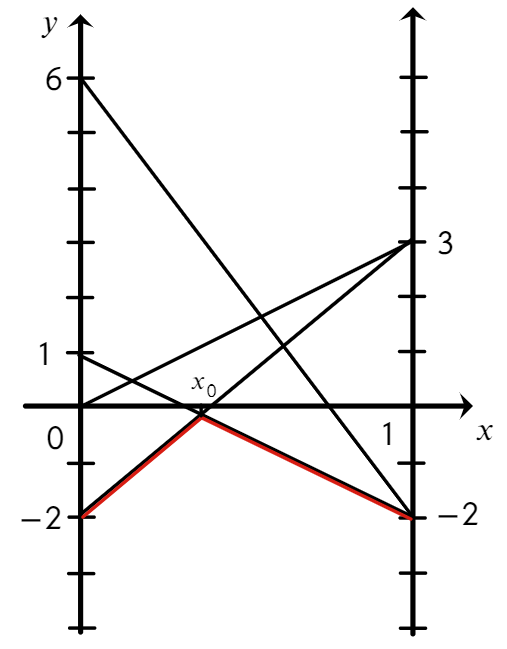
\includegraphics[scale=0.7]{graph1.png}$$ Функция
\(g(x) = \min_{j\in\{1,2,3,4\}} g_j(x)\) есть функция выигрышей игрока
1. Рисуем график \(y=g(x)\) как нижнюю огибающую семейчтва прямых
\(y=g_j(x)\). Стремясь максимизировать свой выигрыщ, игрок 1 должен
найти точку \(x_0\) максимума функции \(g(x)\). Тогда \((x_0,1-x_0)\)
есть оптимальная стратегия игрока 1, \(g(x_0)\) есть цена игры
\(\nu(A_1)\).

Точку \(x_0\) можно вычислить как точку пересечения прямых \(y=g_2(x)\)
и \(y=g_3(x)\). Тогда \[3x_0 -2(1-x_0) = -2x_0 + (1-x_0).\] Выражая
отсюда \(x_0\), получим \[x_0 = \dfrac38.\] Отсюда оптимальная смешанная
стратегия игрока 1 \[p^0 = \left(\dfrac38, \dfrac58\right).\] А цена
игры высиялется как значение \(g_2(x_0)\) или \(g_3(x_0)\):
\[\nu(A_1)=g_2(x_0) = g_3(x_0) = -\dfrac18.\] Теперь вычислим стратегию
игрока 2. Использование неактивных стратегий не может увеличить выигрыш
игрока 2. Если игрок 2 откажется от любой своей неактивной стратегии, то
функция проигрышей игрока 1 может измениться, но минимум новой функции
будет достигаться в той же самой точке \(x_0\). Следовательно, можно
считать, что игрок 1 применяет свои неактивные стратегии с нулевой
вероятностью. В данном случае активными являются стратегии 2 и 3, а
неактивными -- 1 и 4. Тогда \[q_1 = q_4 = 0,\quad q_3 = 1-q_2.\] Найдем
\(q^0\), решая игру с учесенной матрицей
\[A' = \begin{bmatrix} 3 & -2 \\ -2 & 1\end{bmatrix},\] которая
получается путем обрасывания столбцов матрицы, соответствующих
неактивным стратегиям 1 и 4.

Зная, что \(q_3 = 1-q_2\), по первой строке матрицы \(A'\) мы можем
построить уравнение \[3q_2 - 2(1-q_2) = -\dfrac18 = \nu(A_1).\] Таким
образом, \[q_2 = \dfrac38.\] А отсюда имеем оптимальную стратегию игрока
2 равную \[q^0 = \left(0, \dfrac38, \dfrac58, 0\right)\]

    \subsection{\texorpdfstring{Игра с матрицей
\(A_2\)}{Игра с матрицей A\_2}}\label{ux438ux433ux440ux430-ux441-ux43cux430ux442ux440ux438ux446ux435ux439-a_2}

Найдем решение игры для матрицы \(A_2\).
\[A_2 = \begin{bmatrix} 2 & 3 \\ 6 & -2 \\ 0 & 2\end{bmatrix}.\] Нижняя
цена игры:
\[\alpha(A_2)=\max\limits_{1\leq j\leq 4}\min\limits_{1\leq i\leq 2}a_{ij}=2.\]
Верхняя цена игры:
\[\beta(A_2)=\min\limits_{1\leq i\leq 2}\max\limits_{1\leq j\leq 4}a_{ij}=3.\]

    \begin{tcolorbox}[breakable, size=fbox, boxrule=1pt, pad at break*=1mm,colback=cellbackground, colframe=cellborder]
\prompt{In}{incolor}{52}{\boxspacing}
\begin{Verbatim}[commandchars=\\\{\}]
\PY{n}{A\PYZus{}2} \PY{o}{=} \PY{n}{np}\PY{o}{.}\PY{n}{array}\PY{p}{(}\PY{p}{[}\PY{p}{[}\PY{l+m+mi}{2}\PY{p}{,} \PY{l+m+mi}{3}\PY{p}{]}\PY{p}{,}
                \PY{p}{[}\PY{l+m+mi}{6}\PY{p}{,} \PY{o}{\PYZhy{}}\PY{l+m+mi}{2}\PY{p}{]}\PY{p}{,}
                \PY{p}{[}\PY{l+m+mi}{0}\PY{p}{,} \PY{l+m+mi}{2}\PY{p}{]}\PY{p}{]}\PY{p}{)}

\PY{n}{lower\PYZus{}bound\PYZus{}price}\PY{p}{(}\PY{n}{A\PYZus{}2}\PY{p}{)}
\end{Verbatim}
\end{tcolorbox}

            \begin{tcolorbox}[breakable, size=fbox, boxrule=.5pt, pad at break*=1mm, opacityfill=0]
\prompt{Out}{outcolor}{52}{\boxspacing}
\begin{Verbatim}[commandchars=\\\{\}]
2
\end{Verbatim}
\end{tcolorbox}
        
    \begin{tcolorbox}[breakable, size=fbox, boxrule=1pt, pad at break*=1mm,colback=cellbackground, colframe=cellborder]
\prompt{In}{incolor}{53}{\boxspacing}
\begin{Verbatim}[commandchars=\\\{\}]
\PY{n}{upper\PYZus{}bound\PYZus{}price}\PY{p}{(}\PY{n}{A\PYZus{}2}\PY{p}{)}
\end{Verbatim}
\end{tcolorbox}

            \begin{tcolorbox}[breakable, size=fbox, boxrule=.5pt, pad at break*=1mm, opacityfill=0]
\prompt{Out}{outcolor}{53}{\boxspacing}
\begin{Verbatim}[commandchars=\\\{\}]
3
\end{Verbatim}
\end{tcolorbox}
        
    Таким образом, \(\alpha(A_2)\neq \beta(A_2)\). Решать задачу будем в
смешанных стратегиях графическим методом.

Предполагаем, что игрок 2 использует свою смешанную стратегию
\[q^0 = (q_1, q_2)^T = (x, 1-x)^T,\] а игрок 1 использует свою чистую
стратегию \(i\). Тогда средний выигрыш игрока 1 2 равен
\[g_i(x) = x a_{i1} + (1-x) a_{i2}.\] Чтобы нарисовать графики функций
\(y = g_i(x)\) на координатной плоскости \((x,y)\), мы проводим две
вертикальных координатных оси, проходящие через точки \(x=0\) и \(x=1\).

Затем рисуем графики функций \[y = g_1(x) = 2x + 3(1-x),\]
\[y = g_2(x) = 6x -2(1-x),\] \[y = g_3(x) = 2(1-x),\]
$$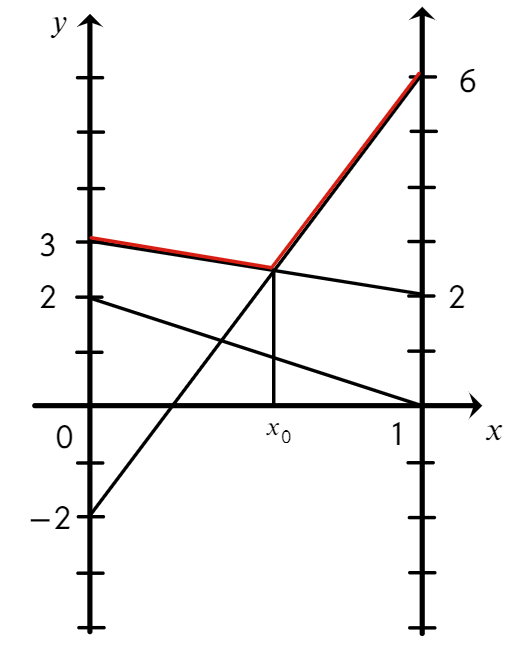
\includegraphics[scale=0.5]{graph2.png}$$ Функция
\(g(x) = \max_{i\in\{1,2,3\}} g_i(x)\) есть функция проигрышей игрока 2.
Рисуем график \(y=g(x)\) как нижнюю огибающую семейчтва прямых
\(y=g_j(x)\). Стремясь минимизировать свой проигрыш, игрок 2 должен
найти точку \(x_0\) минимума функции \(g(x)\). Тогда \((x_0,1-x_0)\)
есть оптимальная стратегия игрока 1, \(g(x_0)\) есть цена игры
\(\nu(A_2)\).

Точку \(x_0\) можно вычислить как точку пересечения прямых \(y=g_1(x)\)
и \(y=g_2(x)\). Тогда \[2x_0  + 3(1-x_0) = 6x_0 -2(1-x_0).\] Выражая
отсюда \(x_0\), получим \[x_0 = \dfrac59.\] Отсюда оптимальная смешанная
стратегия игрока 2 \[q^0 = \left(\dfrac59, \dfrac49\right).\] А цена
игры вычисляется как значение \(g_1(x_0)\) или \(g_2(x_0)\):
\[\nu(A_2)=g_1(x_0) = g_2(x_0) = \dfrac{22}9.\] Теперь вычислим
стратегию игрока 1. В данном случае активными являются стратегии 1 и 2,
а неактивными -- 3. Тогда \[p_2 = 1-p_1, \quad p_3 = 0.\] Найдем
\(p^0\), решая игру с учесенной матрицей
\[A' = \begin{bmatrix} 2 & 3 \\ 6 & -2\end{bmatrix},\] которая
получается путем обрасывания строки матрицы, соответствующей неактивной
стратегии 3.

Зная, что \(p_2 = 1-p_1\), по первой строке матрицы \(A'\) мы можем
построить уравнение \[2p_1  + 3(1-p_1) = \dfrac{22}9 = \nu(A_2).\] Таким
образом, \[p_1 = \dfrac59.\] А отсюда имеем оптимальную стратегию игрока
1 равную \[p^0 = \left(\dfrac59, \dfrac49, 0\right).
\]

    \section{Задача 3}\label{ux437ux430ux434ux430ux447ux430-3}

    Планирование посева.

\begin{enumerate} 
  \item Фермеру необходимо определить, в каких пропорциях сеять свое поле $5$ культурами, если урожайность этих культур, а, значит, и прибыль, зависят от того, каким будет лето: прохладным и дождливым, нормальным, или жарки и сухим.
  \item Фермер подсчитал чистую прибыль с $1$ га от разных культур в зависимости от погоды:\\
\begin{tabular}{ |p{2.5cm}|p{2cm}|p{2cm}|p{2cm}|p{2cm}|p{2cm}|}
 \hline
  & погода $1$ & погода $2$ & погода $3$ & погода $4$ & погода $5$  \\
 \hline
 Культура 1& 2 & 4 & 1 & 4 & 2\\
  \hline
 Культура 2& 1 & 3 & 2 & 2 & 4\\
  \hline
 Культура 3& 3 & 2 & 5 & 2 & 3\\
  \hline
 Культура 4& 1 & 3 & 2 & 5 & 2\\
  \hline
 Культура 5& 2 & 1 & 3 & 3 & 2\\
 \hline
\end{tabular}
\item здесь  фермера нет реального противника.
\item Но, если фермер планирует свою деятельность в расчете на наихудшие погодные условия, то можно считать Природу активным субъектом, который пытается создать наихудшую (с точки зрения фермера) погоду.
\item В таком случае, мы можем смоделировать задачу фермера как матричную игру, в которой фермер является игроком 1, а Природа -- игроком 2.
\item Матрица $A$ выигрышей в данной игре -- это таблица доходов фермера.
\end{enumerate}

    Построим матрицу, соответствующую условию задачи: \[A = \begin{bmatrix}
 2 & 4 & 1 & 4 & 2\\
1 & 3 & 2 & 2 & 4\\
3 & 2 & 5 & 2 & 3\\
1 & 3 & 2 & 5 & 2\\
2 & 1 & 3 & 3 & 2\\
\end{bmatrix}.\] Вычислим нижнюю и верхнюю цены игры.

    \begin{tcolorbox}[breakable, size=fbox, boxrule=1pt, pad at break*=1mm,colback=cellbackground, colframe=cellborder]
\prompt{In}{incolor}{59}{\boxspacing}
\begin{Verbatim}[commandchars=\\\{\}]
\PY{n}{A} \PY{o}{=} \PY{n}{np}\PY{o}{.}\PY{n}{array}\PY{p}{(}\PY{p}{[}\PY{p}{[}\PY{l+m+mi}{2}\PY{p}{,} \PY{l+m+mi}{4}\PY{p}{,} \PY{l+m+mi}{1}\PY{p}{,} \PY{l+m+mi}{4}\PY{p}{,} \PY{l+m+mi}{2}\PY{p}{]}\PY{p}{,}
              \PY{p}{[}\PY{l+m+mi}{1}\PY{p}{,} \PY{l+m+mi}{3}\PY{p}{,} \PY{l+m+mi}{2}\PY{p}{,} \PY{l+m+mi}{2}\PY{p}{,} \PY{l+m+mi}{4}\PY{p}{]}\PY{p}{,}
              \PY{p}{[}\PY{l+m+mi}{3}\PY{p}{,} \PY{l+m+mi}{2}\PY{p}{,} \PY{l+m+mi}{5}\PY{p}{,} \PY{l+m+mi}{2}\PY{p}{,} \PY{l+m+mi}{3}\PY{p}{]}\PY{p}{,}
              \PY{p}{[}\PY{l+m+mi}{1}\PY{p}{,} \PY{l+m+mi}{3}\PY{p}{,} \PY{l+m+mi}{2}\PY{p}{,} \PY{l+m+mi}{5}\PY{p}{,} \PY{l+m+mi}{2}\PY{p}{]}\PY{p}{,}
              \PY{p}{[}\PY{l+m+mi}{2}\PY{p}{,} \PY{l+m+mi}{1}\PY{p}{,} \PY{l+m+mi}{3}\PY{p}{,} \PY{l+m+mi}{3}\PY{p}{,} \PY{l+m+mi}{2}\PY{p}{]}\PY{p}{]}\PY{p}{)}

\PY{n}{lower\PYZus{}bound\PYZus{}price}\PY{p}{(}\PY{n}{A}\PY{p}{)}
\end{Verbatim}
\end{tcolorbox}

            \begin{tcolorbox}[breakable, size=fbox, boxrule=.5pt, pad at break*=1mm, opacityfill=0]
\prompt{Out}{outcolor}{59}{\boxspacing}
\begin{Verbatim}[commandchars=\\\{\}]
2
\end{Verbatim}
\end{tcolorbox}
        
    \begin{tcolorbox}[breakable, size=fbox, boxrule=1pt, pad at break*=1mm,colback=cellbackground, colframe=cellborder]
\prompt{In}{incolor}{58}{\boxspacing}
\begin{Verbatim}[commandchars=\\\{\}]
\PY{n}{upper\PYZus{}bound\PYZus{}price}\PY{p}{(}\PY{n}{A}\PY{p}{)}
\end{Verbatim}
\end{tcolorbox}

            \begin{tcolorbox}[breakable, size=fbox, boxrule=.5pt, pad at break*=1mm, opacityfill=0]
\prompt{Out}{outcolor}{58}{\boxspacing}
\begin{Verbatim}[commandchars=\\\{\}]
3
\end{Verbatim}
\end{tcolorbox}
        
    Таким образом, \(\alpha(A) = 2 < 3 = \beta(A)\), то есть игра не имеет
решения в чистых стратегиях.

Решим игру в смешанныз стратегиях. Поскольку \(\alpha = 2>0\), то
матрицу \(A\) не нужно модифицировать.

Сведем решение матричной игры к решению задачи линейного
программирования. Запишем получившуюся задачу линейного
программирования: \[x_1 + x_2 + x_3 + x_4 + x_5 \to \max\]
\[\begin{cases}
2x_1 +4x_2 +x_3 +4x_4 +2x_5 \leq 1,\\
x_1 +3x_2 +2x_3 +2x_4 +4x_5 \leq 1,\\
3x_1 + 2x_2 + 5x_3 + 2x_4 + 3x_5 \leq 1,\\
x_1 + 3x_2 + 2x_3 + 5x_4 + 2x_5 \leq 1,\\
2x_1 + 1x_2 + 3x_3 + 3x_4 + 2x_5 \leq 1,\\
\end{cases}\] \[x_1, x_2, x_3, x_4, x_5 \geq 0.\]

С помощью библиотеки OR-Tools найдем решение данной задачи линейного
программирования

    \begin{tcolorbox}[breakable, size=fbox, boxrule=1pt, pad at break*=1mm,colback=cellbackground, colframe=cellborder]
\prompt{In}{incolor}{73}{\boxspacing}
\begin{Verbatim}[commandchars=\\\{\}]
\PY{c+ch}{\PYZsh{}!pip install ortools}
\end{Verbatim}
\end{tcolorbox}

    \begin{tcolorbox}[breakable, size=fbox, boxrule=1pt, pad at break*=1mm,colback=cellbackground, colframe=cellborder]
\prompt{In}{incolor}{93}{\boxspacing}
\begin{Verbatim}[commandchars=\\\{\}]
\PY{k+kn}{from} \PY{n+nn}{ortools}\PY{n+nn}{.}\PY{n+nn}{linear\PYZus{}solver} \PY{k+kn}{import} \PY{n}{pywraplp}


\PY{k}{def} \PY{n+nf}{create\PYZus{}data\PYZus{}model}\PY{p}{(}\PY{p}{)}\PY{p}{:}
    \PY{n}{data} \PY{o}{=} \PY{p}{\PYZob{}}\PY{p}{\PYZcb{}}
    \PY{n}{data}\PY{p}{[}\PY{l+s+s2}{\PYZdq{}}\PY{l+s+s2}{constraint\PYZus{}coeffs}\PY{l+s+s2}{\PYZdq{}}\PY{p}{]} \PY{o}{=} \PY{p}{[}
            \PY{p}{[}\PY{l+m+mi}{2}\PY{p}{,} \PY{l+m+mi}{4}\PY{p}{,} \PY{l+m+mi}{1}\PY{p}{,} \PY{l+m+mi}{4}\PY{p}{,} \PY{l+m+mi}{2}\PY{p}{]}\PY{p}{,}
            \PY{p}{[}\PY{l+m+mi}{1}\PY{p}{,} \PY{l+m+mi}{3}\PY{p}{,} \PY{l+m+mi}{2}\PY{p}{,} \PY{l+m+mi}{2}\PY{p}{,} \PY{l+m+mi}{4}\PY{p}{]}\PY{p}{,}
            \PY{p}{[}\PY{l+m+mi}{3}\PY{p}{,} \PY{l+m+mi}{2}\PY{p}{,} \PY{l+m+mi}{5}\PY{p}{,} \PY{l+m+mi}{2}\PY{p}{,} \PY{l+m+mi}{3}\PY{p}{]}\PY{p}{,}
            \PY{p}{[}\PY{l+m+mi}{1}\PY{p}{,} \PY{l+m+mi}{3}\PY{p}{,} \PY{l+m+mi}{2}\PY{p}{,} \PY{l+m+mi}{5}\PY{p}{,} \PY{l+m+mi}{2}\PY{p}{]}\PY{p}{,}
            \PY{p}{[}\PY{l+m+mi}{2}\PY{p}{,} \PY{l+m+mi}{1}\PY{p}{,} \PY{l+m+mi}{3}\PY{p}{,} \PY{l+m+mi}{3}\PY{p}{,} \PY{l+m+mi}{2}\PY{p}{]}\PY{p}{,}
    \PY{p}{]}
    \PY{n}{data}\PY{p}{[}\PY{l+s+s2}{\PYZdq{}}\PY{l+s+s2}{bounds}\PY{l+s+s2}{\PYZdq{}}\PY{p}{]} \PY{o}{=} \PY{p}{[}\PY{l+m+mi}{1}\PY{p}{,} \PY{l+m+mi}{1}\PY{p}{,} \PY{l+m+mi}{1}\PY{p}{,} \PY{l+m+mi}{1}\PY{p}{,} \PY{l+m+mi}{1}\PY{p}{]}
    \PY{n}{data}\PY{p}{[}\PY{l+s+s2}{\PYZdq{}}\PY{l+s+s2}{obj\PYZus{}coeffs}\PY{l+s+s2}{\PYZdq{}}\PY{p}{]} \PY{o}{=} \PY{p}{[}\PY{l+m+mi}{1}\PY{p}{,} \PY{l+m+mi}{1}\PY{p}{,} \PY{l+m+mi}{1}\PY{p}{,} \PY{l+m+mi}{1}\PY{p}{,} \PY{l+m+mi}{1}\PY{p}{]}
    \PY{n}{data}\PY{p}{[}\PY{l+s+s2}{\PYZdq{}}\PY{l+s+s2}{num\PYZus{}vars}\PY{l+s+s2}{\PYZdq{}}\PY{p}{]} \PY{o}{=} \PY{l+m+mi}{5}
    \PY{n}{data}\PY{p}{[}\PY{l+s+s2}{\PYZdq{}}\PY{l+s+s2}{num\PYZus{}constraints}\PY{l+s+s2}{\PYZdq{}}\PY{p}{]} \PY{o}{=} \PY{l+m+mi}{5}
    \PY{k}{return} \PY{n}{data}


\PY{k}{def} \PY{n+nf}{LinearProgramming}\PY{p}{(}\PY{p}{)}\PY{p}{:}
    \PY{n}{data} \PY{o}{=} \PY{n}{create\PYZus{}data\PYZus{}model}\PY{p}{(}\PY{p}{)}
    \PY{n}{solver} \PY{o}{=} \PY{n}{pywraplp}\PY{o}{.}\PY{n}{Solver}\PY{o}{.}\PY{n}{CreateSolver}\PY{p}{(}\PY{l+s+s2}{\PYZdq{}}\PY{l+s+s2}{GLOP}\PY{l+s+s2}{\PYZdq{}}\PY{p}{)}
    \PY{k}{if} \PY{o+ow}{not} \PY{n}{solver}\PY{p}{:}
        \PY{k}{return}

    \PY{n}{infinity} \PY{o}{=} \PY{n}{solver}\PY{o}{.}\PY{n}{infinity}\PY{p}{(}\PY{p}{)}
    \PY{n}{x} \PY{o}{=} \PY{p}{\PYZob{}}\PY{p}{\PYZcb{}}
    \PY{k}{for} \PY{n}{j} \PY{o+ow}{in} \PY{n+nb}{range}\PY{p}{(}\PY{n}{data}\PY{p}{[}\PY{l+s+s2}{\PYZdq{}}\PY{l+s+s2}{num\PYZus{}vars}\PY{l+s+s2}{\PYZdq{}}\PY{p}{]}\PY{p}{)}\PY{p}{:}
        \PY{n}{x}\PY{p}{[}\PY{n}{j}\PY{p}{]} \PY{o}{=} \PY{n}{solver}\PY{o}{.}\PY{n}{IntVar}\PY{p}{(}\PY{l+m+mi}{0}\PY{p}{,} \PY{n}{infinity}\PY{p}{,} \PY{l+s+s2}{\PYZdq{}}\PY{l+s+s2}{x[}\PY{l+s+si}{\PYZpc{}i}\PY{l+s+s2}{]}\PY{l+s+s2}{\PYZdq{}} \PY{o}{\PYZpc{}} \PY{p}{(}\PY{n}{j}\PY{o}{+}\PY{l+m+mi}{1}\PY{p}{)}\PY{p}{)}

    \PY{k}{for} \PY{n}{i} \PY{o+ow}{in} \PY{n+nb}{range}\PY{p}{(}\PY{n}{data}\PY{p}{[}\PY{l+s+s1}{\PYZsq{}}\PY{l+s+s1}{num\PYZus{}constraints}\PY{l+s+s1}{\PYZsq{}}\PY{p}{]}\PY{p}{)}\PY{p}{:}
        \PY{n}{constraint\PYZus{}expr} \PY{o}{=} \PY{p}{[}\PY{n}{data}\PY{p}{[}\PY{l+s+s1}{\PYZsq{}}\PY{l+s+s1}{constraint\PYZus{}coeffs}\PY{l+s+s1}{\PYZsq{}}\PY{p}{]}\PY{p}{[}\PY{n}{i}\PY{p}{]}\PY{p}{[}\PY{n}{j}\PY{p}{]} \PY{o}{*} \PY{n}{x}\PY{p}{[}\PY{n}{j}\PY{p}{]} \PY{k}{for} \PY{n}{j} \PY{o+ow}{in} \PY{n+nb}{range}\PY{p}{(}\PY{n}{data}\PY{p}{[}\PY{l+s+s1}{\PYZsq{}}\PY{l+s+s1}{num\PYZus{}vars}\PY{l+s+s1}{\PYZsq{}}\PY{p}{]}\PY{p}{)}\PY{p}{]}
        \PY{n}{solver}\PY{o}{.}\PY{n}{Add}\PY{p}{(}\PY{n+nb}{sum}\PY{p}{(}\PY{n}{constraint\PYZus{}expr}\PY{p}{)} \PY{o}{\PYZlt{}}\PY{o}{=} \PY{n}{data}\PY{p}{[}\PY{l+s+s1}{\PYZsq{}}\PY{l+s+s1}{bounds}\PY{l+s+s1}{\PYZsq{}}\PY{p}{]}\PY{p}{[}\PY{n}{i}\PY{p}{]}\PY{p}{)}

    \PY{n}{objective} \PY{o}{=} \PY{n}{solver}\PY{o}{.}\PY{n}{Objective}\PY{p}{(}\PY{p}{)}
    \PY{k}{for} \PY{n}{j} \PY{o+ow}{in} \PY{n+nb}{range}\PY{p}{(}\PY{n}{data}\PY{p}{[}\PY{l+s+s2}{\PYZdq{}}\PY{l+s+s2}{num\PYZus{}vars}\PY{l+s+s2}{\PYZdq{}}\PY{p}{]}\PY{p}{)}\PY{p}{:}
        \PY{n}{obj\PYZus{}expr} \PY{o}{=} \PY{p}{[}\PY{n}{data}\PY{p}{[}\PY{l+s+s1}{\PYZsq{}}\PY{l+s+s1}{obj\PYZus{}coeffs}\PY{l+s+s1}{\PYZsq{}}\PY{p}{]}\PY{p}{[}\PY{n}{j}\PY{p}{]} \PY{o}{*} \PY{n}{x}\PY{p}{[}\PY{n}{j}\PY{p}{]} \PY{k}{for} \PY{n}{j} \PY{o+ow}{in} \PY{n+nb}{range}\PY{p}{(}\PY{n}{data}\PY{p}{[}\PY{l+s+s1}{\PYZsq{}}\PY{l+s+s1}{num\PYZus{}vars}\PY{l+s+s1}{\PYZsq{}}\PY{p}{]}\PY{p}{)}\PY{p}{]}
    \PY{n}{solver}\PY{o}{.}\PY{n}{Maximize}\PY{p}{(}\PY{n}{solver}\PY{o}{.}\PY{n}{Sum}\PY{p}{(}\PY{n}{obj\PYZus{}expr}\PY{p}{)}\PY{p}{)}

    \PY{n+nb}{print}\PY{p}{(}\PY{l+s+sa}{f}\PY{l+s+s2}{\PYZdq{}}\PY{l+s+s2}{Solving with }\PY{l+s+si}{\PYZob{}}\PY{n}{solver}\PY{o}{.}\PY{n}{SolverVersion}\PY{p}{(}\PY{p}{)}\PY{l+s+si}{\PYZcb{}}\PY{l+s+s2}{\PYZdq{}}\PY{p}{)}
    \PY{n}{status} \PY{o}{=} \PY{n}{solver}\PY{o}{.}\PY{n}{Solve}\PY{p}{(}\PY{p}{)}

    \PY{k}{if} \PY{n}{status} \PY{o}{==} \PY{n}{pywraplp}\PY{o}{.}\PY{n}{Solver}\PY{o}{.}\PY{n}{OPTIMAL}\PY{p}{:}
        \PY{n+nb}{print}\PY{p}{(}\PY{l+s+s2}{\PYZdq{}}\PY{l+s+s2}{Objective value =}\PY{l+s+s2}{\PYZdq{}}\PY{p}{,} \PY{n}{solver}\PY{o}{.}\PY{n}{Objective}\PY{p}{(}\PY{p}{)}\PY{o}{.}\PY{n}{Value}\PY{p}{(}\PY{p}{)}\PY{p}{)}
        \PY{k}{for} \PY{n}{j} \PY{o+ow}{in} \PY{n+nb}{range}\PY{p}{(}\PY{n}{data}\PY{p}{[}\PY{l+s+s2}{\PYZdq{}}\PY{l+s+s2}{num\PYZus{}vars}\PY{l+s+s2}{\PYZdq{}}\PY{p}{]}\PY{p}{)}\PY{p}{:}
            \PY{n+nb}{print}\PY{p}{(}\PY{n}{x}\PY{p}{[}\PY{n}{j}\PY{p}{]}\PY{o}{.}\PY{n}{name}\PY{p}{(}\PY{p}{)}\PY{p}{,} \PY{l+s+s2}{\PYZdq{}}\PY{l+s+s2}{ = }\PY{l+s+s2}{\PYZdq{}}\PY{p}{,} \PY{n}{x}\PY{p}{[}\PY{n}{j}\PY{p}{]}\PY{o}{.}\PY{n}{solution\PYZus{}value}\PY{p}{(}\PY{p}{)}\PY{p}{)}
        \PY{n+nb}{print}\PY{p}{(}\PY{p}{)}
        \PY{n+nb}{print}\PY{p}{(}\PY{l+s+sa}{f}\PY{l+s+s2}{\PYZdq{}}\PY{l+s+s2}{Problem solved in }\PY{l+s+si}{\PYZob{}}\PY{n}{solver}\PY{o}{.}\PY{n}{iterations}\PY{p}{(}\PY{p}{)}\PY{l+s+si}{:}\PY{l+s+s2}{d}\PY{l+s+si}{\PYZcb{}}\PY{l+s+s2}{ iterations}\PY{l+s+s2}{\PYZdq{}}\PY{p}{)}
    \PY{k}{else}\PY{p}{:}
        \PY{n+nb}{print}\PY{p}{(}\PY{l+s+s2}{\PYZdq{}}\PY{l+s+s2}{The problem does not have an optimal solution.}\PY{l+s+s2}{\PYZdq{}}\PY{p}{)}

\PY{n}{LinearProgramming}\PY{p}{(}\PY{p}{)}
\end{Verbatim}
\end{tcolorbox}

    \begin{Verbatim}[commandchars=\\\{\}]
Solving with Glop solver v9.9.3963
Objective value = 0.375
x[1]  =  0.25
x[2]  =  0.125
x[3]  =  0.0
x[4]  =  0.0
x[5]  =  0.0

Problem solved in 2 iterations
    \end{Verbatim}

    Составим задачу линейного программирования двойственную к составленной
нами ранее \[y_1 + y_2 + y_3 + y_4 + y_5 \to \min\] \[\begin{cases}
2y_1 +4y_2 +y_3 +4y_4 +2y_5 \geq 1,\\
y_1 +3y_2 +2y_3 +2y_4 +4y_5 \geq 1,\\
3y_1 + 2y_2 + 5y_3 + 2y_4 + 3y_5 \geq 1,\\
y_1 + 3y_2 + 2y_3 + 5y_4 + 2y_5 \geq 1,\\
2y_1 + 1y_2 + 3y_3 + 3y_4 + 2y_5 \geq 1,\\
\end{cases}\] \[y_1, y_2, y_3, y_4, y_5 \geq 0.\] Также с помощью
OR-Tools найдем решение двойственной задачи ЛП.

    \begin{tcolorbox}[breakable, size=fbox, boxrule=1pt, pad at break*=1mm,colback=cellbackground, colframe=cellborder]
\prompt{In}{incolor}{94}{\boxspacing}
\begin{Verbatim}[commandchars=\\\{\}]
\PY{k}{def} \PY{n+nf}{DualLinearProgramming}\PY{p}{(}\PY{p}{)}\PY{p}{:}
    \PY{n}{data} \PY{o}{=} \PY{n}{create\PYZus{}data\PYZus{}model}\PY{p}{(}\PY{p}{)}
    \PY{n}{solver} \PY{o}{=} \PY{n}{pywraplp}\PY{o}{.}\PY{n}{Solver}\PY{o}{.}\PY{n}{CreateSolver}\PY{p}{(}\PY{l+s+s2}{\PYZdq{}}\PY{l+s+s2}{GLOP}\PY{l+s+s2}{\PYZdq{}}\PY{p}{)}
    \PY{k}{if} \PY{o+ow}{not} \PY{n}{solver}\PY{p}{:}
        \PY{k}{return}

    \PY{n}{infinity} \PY{o}{=} \PY{n}{solver}\PY{o}{.}\PY{n}{infinity}\PY{p}{(}\PY{p}{)}
    \PY{n}{y} \PY{o}{=} \PY{p}{\PYZob{}}\PY{p}{\PYZcb{}}
    \PY{k}{for} \PY{n}{j} \PY{o+ow}{in} \PY{n+nb}{range}\PY{p}{(}\PY{n}{data}\PY{p}{[}\PY{l+s+s2}{\PYZdq{}}\PY{l+s+s2}{num\PYZus{}vars}\PY{l+s+s2}{\PYZdq{}}\PY{p}{]}\PY{p}{)}\PY{p}{:}
        \PY{n}{y}\PY{p}{[}\PY{n}{j}\PY{p}{]} \PY{o}{=} \PY{n}{solver}\PY{o}{.}\PY{n}{IntVar}\PY{p}{(}\PY{l+m+mi}{0}\PY{p}{,} \PY{n}{infinity}\PY{p}{,} \PY{l+s+s2}{\PYZdq{}}\PY{l+s+s2}{y[}\PY{l+s+si}{\PYZpc{}i}\PY{l+s+s2}{]}\PY{l+s+s2}{\PYZdq{}} \PY{o}{\PYZpc{}} \PY{p}{(}\PY{n}{j}\PY{o}{+}\PY{l+m+mi}{1}\PY{p}{)}\PY{p}{)}

    \PY{k}{for} \PY{n}{i} \PY{o+ow}{in} \PY{n+nb}{range}\PY{p}{(}\PY{n}{data}\PY{p}{[}\PY{l+s+s1}{\PYZsq{}}\PY{l+s+s1}{num\PYZus{}constraints}\PY{l+s+s1}{\PYZsq{}}\PY{p}{]}\PY{p}{)}\PY{p}{:}
        \PY{n}{constraint\PYZus{}expr} \PY{o}{=} \PY{p}{[}\PY{n}{data}\PY{p}{[}\PY{l+s+s1}{\PYZsq{}}\PY{l+s+s1}{constraint\PYZus{}coeffs}\PY{l+s+s1}{\PYZsq{}}\PY{p}{]}\PY{p}{[}\PY{n}{i}\PY{p}{]}\PY{p}{[}\PY{n}{j}\PY{p}{]} \PY{o}{*} \PY{n}{y}\PY{p}{[}\PY{n}{j}\PY{p}{]} \PY{k}{for} \PY{n}{j} \PY{o+ow}{in} \PY{n+nb}{range}\PY{p}{(}\PY{n}{data}\PY{p}{[}\PY{l+s+s1}{\PYZsq{}}\PY{l+s+s1}{num\PYZus{}vars}\PY{l+s+s1}{\PYZsq{}}\PY{p}{]}\PY{p}{)}\PY{p}{]}
        \PY{n}{solver}\PY{o}{.}\PY{n}{Add}\PY{p}{(}\PY{n+nb}{sum}\PY{p}{(}\PY{n}{constraint\PYZus{}expr}\PY{p}{)} \PY{o}{\PYZgt{}}\PY{o}{=} \PY{n}{data}\PY{p}{[}\PY{l+s+s1}{\PYZsq{}}\PY{l+s+s1}{bounds}\PY{l+s+s1}{\PYZsq{}}\PY{p}{]}\PY{p}{[}\PY{n}{i}\PY{p}{]}\PY{p}{)}

    \PY{n}{objective} \PY{o}{=} \PY{n}{solver}\PY{o}{.}\PY{n}{Objective}\PY{p}{(}\PY{p}{)}
    \PY{k}{for} \PY{n}{j} \PY{o+ow}{in} \PY{n+nb}{range}\PY{p}{(}\PY{n}{data}\PY{p}{[}\PY{l+s+s2}{\PYZdq{}}\PY{l+s+s2}{num\PYZus{}vars}\PY{l+s+s2}{\PYZdq{}}\PY{p}{]}\PY{p}{)}\PY{p}{:}
        \PY{n}{obj\PYZus{}expr} \PY{o}{=} \PY{p}{[}\PY{n}{data}\PY{p}{[}\PY{l+s+s1}{\PYZsq{}}\PY{l+s+s1}{obj\PYZus{}coeffs}\PY{l+s+s1}{\PYZsq{}}\PY{p}{]}\PY{p}{[}\PY{n}{j}\PY{p}{]} \PY{o}{*} \PY{n}{y}\PY{p}{[}\PY{n}{j}\PY{p}{]} \PY{k}{for} \PY{n}{j} \PY{o+ow}{in} \PY{n+nb}{range}\PY{p}{(}\PY{n}{data}\PY{p}{[}\PY{l+s+s1}{\PYZsq{}}\PY{l+s+s1}{num\PYZus{}vars}\PY{l+s+s1}{\PYZsq{}}\PY{p}{]}\PY{p}{)}\PY{p}{]}
    \PY{n}{solver}\PY{o}{.}\PY{n}{Minimize}\PY{p}{(}\PY{n}{solver}\PY{o}{.}\PY{n}{Sum}\PY{p}{(}\PY{n}{obj\PYZus{}expr}\PY{p}{)}\PY{p}{)}

    \PY{n+nb}{print}\PY{p}{(}\PY{l+s+sa}{f}\PY{l+s+s2}{\PYZdq{}}\PY{l+s+s2}{Solving with }\PY{l+s+si}{\PYZob{}}\PY{n}{solver}\PY{o}{.}\PY{n}{SolverVersion}\PY{p}{(}\PY{p}{)}\PY{l+s+si}{\PYZcb{}}\PY{l+s+s2}{\PYZdq{}}\PY{p}{)}
    \PY{n}{status} \PY{o}{=} \PY{n}{solver}\PY{o}{.}\PY{n}{Solve}\PY{p}{(}\PY{p}{)}

    \PY{k}{if} \PY{n}{status} \PY{o}{==} \PY{n}{pywraplp}\PY{o}{.}\PY{n}{Solver}\PY{o}{.}\PY{n}{OPTIMAL}\PY{p}{:}
        \PY{n+nb}{print}\PY{p}{(}\PY{l+s+s2}{\PYZdq{}}\PY{l+s+s2}{Objective value =}\PY{l+s+s2}{\PYZdq{}}\PY{p}{,} \PY{n}{solver}\PY{o}{.}\PY{n}{Objective}\PY{p}{(}\PY{p}{)}\PY{o}{.}\PY{n}{Value}\PY{p}{(}\PY{p}{)}\PY{p}{)}
        \PY{k}{for} \PY{n}{j} \PY{o+ow}{in} \PY{n+nb}{range}\PY{p}{(}\PY{n}{data}\PY{p}{[}\PY{l+s+s2}{\PYZdq{}}\PY{l+s+s2}{num\PYZus{}vars}\PY{l+s+s2}{\PYZdq{}}\PY{p}{]}\PY{p}{)}\PY{p}{:}
            \PY{n+nb}{print}\PY{p}{(}\PY{n}{y}\PY{p}{[}\PY{n}{j}\PY{p}{]}\PY{o}{.}\PY{n}{name}\PY{p}{(}\PY{p}{)}\PY{p}{,} \PY{l+s+s2}{\PYZdq{}}\PY{l+s+s2}{ = }\PY{l+s+s2}{\PYZdq{}}\PY{p}{,} \PY{n}{y}\PY{p}{[}\PY{n}{j}\PY{p}{]}\PY{o}{.}\PY{n}{solution\PYZus{}value}\PY{p}{(}\PY{p}{)}\PY{p}{)}
        \PY{n+nb}{print}\PY{p}{(}\PY{p}{)}
        \PY{n+nb}{print}\PY{p}{(}\PY{l+s+sa}{f}\PY{l+s+s2}{\PYZdq{}}\PY{l+s+s2}{Problem solved in }\PY{l+s+si}{\PYZob{}}\PY{n}{solver}\PY{o}{.}\PY{n}{iterations}\PY{p}{(}\PY{p}{)}\PY{l+s+si}{:}\PY{l+s+s2}{d}\PY{l+s+si}{\PYZcb{}}\PY{l+s+s2}{ iterations}\PY{l+s+s2}{\PYZdq{}}\PY{p}{)}
    \PY{k}{else}\PY{p}{:}
        \PY{n+nb}{print}\PY{p}{(}\PY{l+s+s2}{\PYZdq{}}\PY{l+s+s2}{The problem does not have an optimal solution.}\PY{l+s+s2}{\PYZdq{}}\PY{p}{)}

\PY{n}{DualLinearProgramming}\PY{p}{(}\PY{p}{)}
\end{Verbatim}
\end{tcolorbox}

    \begin{Verbatim}[commandchars=\\\{\}]
Solving with Glop solver v9.9.3963
Objective value = 0.375
y[1]  =  0.0
y[2]  =  0.0
y[3]  =  0.08333333333333338
y[4]  =  0.16666666666666666
y[5]  =  0.12499999999999997

Problem solved in 5 iterations
    \end{Verbatim}

    Итого имеем оптимальное решение исходной и двойственной к ней задач
\[x^0 = \begin{bmatrix} 0.25 \\ 0.125 \\ 0 \\ 0\\ 0\end{bmatrix},\quad y^0 = \begin{bmatrix} 0 \\ 0 \\ \frac{1}{12} \\ \frac{1}{6} \\ \frac{1}8\end{bmatrix}\]
Найдем цену игры:
\[\nu(A) = \dfrac{1}{y_1^0 + y_2^0 + y_3^0 + y_4^0 + y_5^0} = \dfrac{1}{\frac{2}{24} + \frac{4}{24} + \frac{3}{24}} = \dfrac{24}{9}\approx 2.67.\]

Тогда оптимальная стратегия игрока 1 равна
\[p^0 = \nu(A) y^0 = \left(0, 0, \dfrac29, \dfrac49, \dfrac39\right).\]
Оптимальная стратегия игрока 2 (природы) равна
\[q^0 = \nu(A) x^0 = \left(\dfrac23, \dfrac13, 0, 0, 0\right).\]

Таким образом, смешанная стратегия рекомендует фермеру засеять \(2/9\)
поля культурной 3, \(3/9\) культурой 4, \(4/9\) культурой 5. При любой
погоде доход фермера будет не меньшим цены \(\nu(A) = \dfrac{24}9\)
данной игры.

    \section{Задача 4}\label{ux437ux430ux434ux430ux447ux430-4}

    Магазин имеет некоторый запас товаров ассортиментного минимума. Если
запас товаров недостаточен, то необходимо завести его с базы; если запас
превышает спрос, то магазин несет расходы по хранению нереализованного
товара. Пусть спрос на товары лежит в пределах \(S\)
(\(5 \leq S \leq 8\) единиц), расходы по хранению одной единицы товара
составляют \(c\) руб., а расходы по завозу единицы товара \(k\) руб.,
цена за единицу товара составляет \(p\) руб. Составить платежную
матрицу, элементами которой является прибыль магазина (доход от продажи
с учетом расходов по хранению или по завозу). Определить оптимальную
стратегию магазина по завозу товаров, используя критерии Вальда,
Сэвиджа, Гурвица при \(\alpha = 0.5\), Лапласа.

В соответствии с вариантом входные данные:

\begin{itemize}
	\item \(p=350\) -- цена за
	единицу товара;
\item
  \(c=60\) -- расход по хранению одной единицы товара;
\item
  \(k=70\) -- расходы по завозу одной единицы товара.
\end{itemize}

Матрица в общем виде, где по горизонтали необходимое количество товара,
а по вертикали количество товара, которое есть в наличие, при условии,
что количество товара изменяется от \(5\) до \(8\), имеет вид:
\[\begin{bmatrix}
    5p & 6p-k & 7p-2k & 8p-3k\\
    5p-c & 6p & 7p-k & 8p-2k\\
    5p-2c & 6p-c & 7p & 8p-k\\
    5p-3c & 6p-2c & 7p-c & 8p
\end{bmatrix}\]

Вычислим программно вид матрицы при подставленных входных данных:

    \begin{tcolorbox}[breakable, size=fbox, boxrule=1pt, pad at break*=1mm,colback=cellbackground, colframe=cellborder]
\prompt{In}{incolor}{143}{\boxspacing}
\begin{Verbatim}[commandchars=\\\{\}]
\PY{k}{def} \PY{n+nf}{init\PYZus{}matrix}\PY{p}{(}\PY{n}{p}\PY{p}{,} \PY{n}{c}\PY{p}{,} \PY{n}{k}\PY{p}{)}\PY{p}{:}
    \PY{n}{n} \PY{o}{=} \PY{l+m+mi}{4}
    \PY{n}{matrix} \PY{o}{=} \PY{n}{np}\PY{o}{.}\PY{n}{zeros}\PY{p}{(}\PY{p}{(}\PY{n}{n}\PY{p}{,} \PY{n}{n}\PY{p}{)}\PY{p}{)}
    \PY{k}{for} \PY{n}{i} \PY{o+ow}{in} \PY{n+nb}{range}\PY{p}{(}\PY{n}{n}\PY{p}{)}\PY{p}{:}
        \PY{k}{for} \PY{n}{j} \PY{o+ow}{in} \PY{n+nb}{range}\PY{p}{(}\PY{n}{n}\PY{p}{)}\PY{p}{:}
            \PY{k}{if} \PY{n}{i} \PY{o}{==} \PY{n}{j}\PY{p}{:}
                \PY{n}{matrix}\PY{p}{[}\PY{n}{i}\PY{p}{,} \PY{n}{j}\PY{p}{]} \PY{o}{=} \PY{p}{(}\PY{l+m+mi}{5}\PY{o}{+}\PY{n}{i}\PY{p}{)}\PY{o}{*}\PY{n}{p}
            \PY{k}{for} \PY{n}{l} \PY{o+ow}{in} \PY{n+nb}{range}\PY{p}{(}\PY{l+m+mi}{1}\PY{p}{,} \PY{l+m+mi}{4}\PY{p}{)}\PY{p}{:}
                \PY{k}{if} \PY{n}{i} \PY{o}{==} \PY{n}{j}\PY{o}{\PYZhy{}}\PY{n}{l}\PY{p}{:}
                    \PY{n}{matrix}\PY{p}{[}\PY{n}{i}\PY{p}{,} \PY{n}{j}\PY{p}{]} \PY{o}{=} \PY{p}{(}\PY{l+m+mi}{5}\PY{o}{+}\PY{n}{j}\PY{p}{)}\PY{o}{*}\PY{n}{p} \PY{o}{\PYZhy{}} \PY{n}{l}\PY{o}{*}\PY{n}{k}
            \PY{k}{for} \PY{n}{l} \PY{o+ow}{in} \PY{n+nb}{range}\PY{p}{(}\PY{l+m+mi}{1}\PY{p}{,} \PY{l+m+mi}{4}\PY{p}{)}\PY{p}{:}
                \PY{k}{if} \PY{n}{i} \PY{o}{==} \PY{n}{j}\PY{o}{+}\PY{n}{l}\PY{p}{:}
                    \PY{n}{matrix}\PY{p}{[}\PY{n}{i}\PY{p}{,} \PY{n}{j}\PY{p}{]} \PY{o}{=} \PY{p}{(}\PY{l+m+mi}{5}\PY{o}{+}\PY{n}{j}\PY{p}{)}\PY{o}{*}\PY{n}{p} \PY{o}{\PYZhy{}} \PY{n}{l}\PY{o}{*}\PY{n}{c}
    \PY{k}{return} \PY{n}{matrix}
\end{Verbatim}
\end{tcolorbox}

    \begin{tcolorbox}[breakable, size=fbox, boxrule=1pt, pad at break*=1mm,colback=cellbackground, colframe=cellborder]
\prompt{In}{incolor}{184}{\boxspacing}
\begin{Verbatim}[commandchars=\\\{\}]
\PY{n}{C} \PY{o}{=} \PY{n}{init\PYZus{}matrix}\PY{p}{(}\PY{l+m+mi}{300}\PY{p}{,} \PY{l+m+mi}{50}\PY{p}{,} \PY{l+m+mi}{70}\PY{p}{)}
\PY{n}{B} \PY{o}{=} \PY{n}{init\PYZus{}matrix}\PY{p}{(}\PY{l+m+mi}{210}\PY{p}{,} \PY{l+m+mi}{20}\PY{p}{,} \PY{l+m+mi}{60}\PY{p}{)}
\PY{n}{A} \PY{o}{=} \PY{n}{init\PYZus{}matrix}\PY{p}{(}\PY{l+m+mi}{350}\PY{p}{,} \PY{l+m+mi}{60}\PY{p}{,} \PY{l+m+mi}{70}\PY{p}{)}
\PY{n}{A}
\end{Verbatim}
\end{tcolorbox}

            \begin{tcolorbox}[breakable, size=fbox, boxrule=.5pt, pad at break*=1mm, opacityfill=0]
\prompt{Out}{outcolor}{184}{\boxspacing}
\begin{Verbatim}[commandchars=\\\{\}]
array([[1750., 2030., 2310., 2590.],
       [1690., 2100., 2380., 2660.],
       [1630., 2040., 2450., 2730.],
       [1570., 1980., 2390., 2800.]])
\end{Verbatim}
\end{tcolorbox}
        
    Воспользуемся критерием Вальда: \[W=\max\limits_i\min\limits_j a_{ij}.\]
Программно реализуем функцию, которая будет вычислять значение W.

    \begin{tcolorbox}[breakable, size=fbox, boxrule=1pt, pad at break*=1mm,colback=cellbackground, colframe=cellborder]
\prompt{In}{incolor}{158}{\boxspacing}
\begin{Verbatim}[commandchars=\\\{\}]
\PY{k}{def} \PY{n+nf}{W}\PY{p}{(}\PY{n}{A}\PY{p}{)}\PY{p}{:}
        \PY{k}{return} \PY{n}{A}\PY{o}{.}\PY{n}{min}\PY{p}{(}\PY{n}{axis}\PY{o}{=}\PY{l+m+mi}{1}\PY{p}{)}\PY{o}{.}\PY{n}{max}\PY{p}{(}\PY{p}{)}
    
\PY{n}{W}\PY{p}{(}\PY{n}{A}\PY{p}{)}
\end{Verbatim}
\end{tcolorbox}

            \begin{tcolorbox}[breakable, size=fbox, boxrule=.5pt, pad at break*=1mm, opacityfill=0]
\prompt{Out}{outcolor}{158}{\boxspacing}
\begin{Verbatim}[commandchars=\\\{\}]
1750.0
\end{Verbatim}
\end{tcolorbox}
        
    То есть оптимальная стратегия -- завоз 5 единиц.

Воспользуемся критерием Сэвиджа \[S=\min\limits_i\max\limits_j r_{ij}\]
\[b_j=\max\limits_i a_{ij}\] \[r_{ij}=b_j-a_{ij}=a_{\max j}-a_{ij}\]

Составим компьютерный метод, который будем вычислять по соответствующим
формулам матрицу \((r_{ij})\) и находить число \(S\).

    \begin{tcolorbox}[breakable, size=fbox, boxrule=1pt, pad at break*=1mm,colback=cellbackground, colframe=cellborder]
\prompt{In}{incolor}{203}{\boxspacing}
\begin{Verbatim}[commandchars=\\\{\}]
\PY{k}{def} \PY{n+nf}{S}\PY{p}{(}\PY{n}{A}\PY{p}{)}\PY{p}{:}
    \PY{n}{r} \PY{o}{=} \PY{n}{np}\PY{o}{.}\PY{n}{array}\PY{p}{(}\PY{n}{A}\PY{o}{.}\PY{n}{shape}\PY{p}{)}
    \PY{n}{b} \PY{o}{=} \PY{n}{A}\PY{o}{.}\PY{n}{max}\PY{p}{(}\PY{n}{axis}\PY{o}{=}\PY{l+m+mi}{1}\PY{p}{)}
    \PY{n}{r} \PY{o}{=} \PY{n}{np}\PY{o}{.}\PY{n}{array}\PY{p}{(}\PY{p}{[}\PY{n}{b} \PY{k}{for} \PY{n}{\PYZus{}} \PY{o+ow}{in} \PY{n+nb}{range}\PY{p}{(}\PY{l+m+mi}{4}\PY{p}{)}\PY{p}{]}\PY{p}{)} \PY{o}{\PYZhy{}} \PY{n}{A}
    \PY{n}{S} \PY{o}{=} \PY{n}{r}\PY{o}{.}\PY{n}{max}\PY{p}{(}\PY{n}{axis}\PY{o}{=}\PY{l+m+mi}{1}\PY{p}{)}\PY{o}{.}\PY{n}{min}\PY{p}{(}\PY{p}{)}
    \PY{k}{return} \PY{n}{r}\PY{p}{,} \PY{n}{S}
\end{Verbatim}
\end{tcolorbox}

    \begin{tcolorbox}[breakable, size=fbox, boxrule=1pt, pad at break*=1mm,colback=cellbackground, colframe=cellborder]
\prompt{In}{incolor}{204}{\boxspacing}
\begin{Verbatim}[commandchars=\\\{\}]
\PY{n}{S}\PY{p}{(}\PY{n}{A}\PY{p}{)}
\end{Verbatim}
\end{tcolorbox}

            \begin{tcolorbox}[breakable, size=fbox, boxrule=.5pt, pad at break*=1mm, opacityfill=0]
\prompt{Out}{outcolor}{204}{\boxspacing}
\begin{Verbatim}[commandchars=\\\{\}]
(array([[ 840.,  630.,  420.,  210.],
        [ 900.,  560.,  350.,  140.],
        [ 960.,  620.,  280.,   70.],
        [1020.,  680.,  340.,    0.]]),
 840.0)
\end{Verbatim}
\end{tcolorbox}
        
    Таким образом, максимальное значение риска по каждой строке равно
\([840, 900, 960, 1020]\), а значение критерия Сэвиджа равно
\(S = 840\). Отсюда следует, что оптимальная стратегия -- завоз 5
товаров.

Воспользуемся критерием Гурвица (\(\lambda=0.5\)):
\[H=\max\limits_i (\lambda \max\limits_j a_{ij}+(1-\lambda) \min\limits_j a_{ij})\]
Составим программный метод, который возвращает получившийся вектор и
максимальное значение в нем.

    \begin{tcolorbox}[breakable, size=fbox, boxrule=1pt, pad at break*=1mm,colback=cellbackground, colframe=cellborder]
\prompt{In}{incolor}{214}{\boxspacing}
\begin{Verbatim}[commandchars=\\\{\}]
\PY{k}{def} \PY{n+nf}{H}\PY{p}{(}\PY{n}{A}\PY{p}{,} \PY{n}{l}\PY{p}{)}\PY{p}{:}
    \PY{n}{h} \PY{o}{=} \PY{n}{l} \PY{o}{*} \PY{n}{A}\PY{o}{.}\PY{n}{max}\PY{p}{(}\PY{n}{axis}\PY{o}{=}\PY{l+m+mi}{1}\PY{p}{)} \PY{o}{+} \PY{p}{(}\PY{l+m+mi}{1}\PY{o}{\PYZhy{}}\PY{n}{l}\PY{p}{)}\PY{o}{*}\PY{n}{A}\PY{o}{.}\PY{n}{min}\PY{p}{(}\PY{n}{axis}\PY{o}{=}\PY{l+m+mi}{1}\PY{p}{)}
    \PY{k}{return} \PY{n}{h}\PY{p}{,} \PY{n}{h}\PY{o}{.}\PY{n}{max}\PY{p}{(}\PY{p}{)}
\end{Verbatim}
\end{tcolorbox}

    \begin{tcolorbox}[breakable, size=fbox, boxrule=1pt, pad at break*=1mm,colback=cellbackground, colframe=cellborder]
\prompt{In}{incolor}{215}{\boxspacing}
\begin{Verbatim}[commandchars=\\\{\}]
\PY{n}{H}\PY{p}{(}\PY{n}{B}\PY{p}{,} \PY{l+m+mf}{0.5}\PY{p}{)}
\end{Verbatim}
\end{tcolorbox}

            \begin{tcolorbox}[breakable, size=fbox, boxrule=.5pt, pad at break*=1mm, opacityfill=0]
\prompt{Out}{outcolor}{215}{\boxspacing}
\begin{Verbatim}[commandchars=\\\{\}]
(array([1275., 1295., 1315., 1335.]), 1335.0)
\end{Verbatim}
\end{tcolorbox}
        
    Таким образом, вектор равен \([1275, 1295, 1315, 1335]\), а значение
критерия Гурвица равно \(H = 1335\).

Воспользуемся критерием Лапласа:
\[L=\max\limits_{i\in \overline{1,m}}\frac{1}{n}\sum\limits_{j=1}^n a_{ij}.\]
Составим программный метод, который возвращает получившийся вектор и
максимальное значение в нем.

    \begin{tcolorbox}[breakable, size=fbox, boxrule=1pt, pad at break*=1mm,colback=cellbackground, colframe=cellborder]
\prompt{In}{incolor}{221}{\boxspacing}
\begin{Verbatim}[commandchars=\\\{\}]
\PY{k}{def} \PY{n+nf}{L}\PY{p}{(}\PY{n}{A}\PY{p}{)}\PY{p}{:}
    \PY{n}{l} \PY{o}{=} \PY{n}{np}\PY{o}{.}\PY{n}{mean}\PY{p}{(}\PY{n}{A}\PY{p}{,} \PY{n}{axis}\PY{o}{=}\PY{l+m+mi}{1}\PY{p}{)}
    \PY{k}{return} \PY{n}{l}\PY{p}{,} \PY{n}{l}\PY{o}{.}\PY{n}{max}\PY{p}{(}\PY{p}{)}
\end{Verbatim}
\end{tcolorbox}

    \begin{tcolorbox}[breakable, size=fbox, boxrule=1pt, pad at break*=1mm,colback=cellbackground, colframe=cellborder]
\prompt{In}{incolor}{223}{\boxspacing}
\begin{Verbatim}[commandchars=\\\{\}]
\PY{n}{L}\PY{p}{(}\PY{n}{A}\PY{p}{)}
\end{Verbatim}
\end{tcolorbox}

            \begin{tcolorbox}[breakable, size=fbox, boxrule=.5pt, pad at break*=1mm, opacityfill=0]
\prompt{Out}{outcolor}{223}{\boxspacing}
\begin{Verbatim}[commandchars=\\\{\}]
(array([2170. , 2207.5, 2212.5, 2185. ]), 2212.5)
\end{Verbatim}
\end{tcolorbox}
        
    Таким образом, вектор равен \([2170, 2207.5, 2212.5, 2185]\), а значение
критерия Лапласа равно \(L = 2212.5\).


    % Add a bibliography block to the postdoc
    
    
    
\end{document}
